% !TeX root = main.tex
%Dies ist die Hauptseite des Dokumentes. Es werden u. a. alle Kapitel,
%Einstellung im Header eingebunden.  Veränderungen müssen in folgenden Dateien
%vorgenommen werden:
      %- config.tex
      %- einzelne Kapitel (evtl. erweitern)

%Hier sind alle Einstellungen enthalten, die sich auf das Seiten- und
%Dokumentenlayout beziehen

\documentclass[
  11pt,                   % Schriftgröße
  DIV12,
  german,                 % für Umlaute, Silbentrennung etc.
  oneside,                % einseitiges Dokument
  titlepage,              % es wird eine Titelseite verwendet
  parskip=half,           % Abstand zwischen Absätzen (halbe Zeile)
  headings=normal,        % Größe der Überschriften verkleinern
  captions=tableheading,  % Beschriftung von Tabellen unterhalb ausgeben
  final                   % Status des Dokuments (final/draft)
]{scrreprt}               %


%------Ändern von Schriftschnitten - (Muss ganz am Anfang stehen !) ------------
\usepackage{fix-cm}


%------Umlaute -----------------------------------------------------------------
%   Umlaute/Sonderzeichen wie äüöß können direkt im Quelltext verwenden werden.
%    Erlaubt automatische Trennung von Worten mit Umlauten.
\usepackage[T1]{fontenc}
\usepackage[utf8]{inputenc}

%------Anpassung der Landessprache----------------------------------------------
\usepackage[ngerman]{babel}

%------Einfache Definition der Zeilenabstände und Seitenränder------------------
\usepackage{geometry}
\usepackage{setspace}

%------Schriftgrößenanpassung von einzelnen Textpassagen------------------------
\usepackage{relsize}

%------Trennlinien in Kopf- und Fusszeile
\usepackage[headsepline, footsepline, ilines]{scrlayer-scrpage}

%------Grafiken und Farben -----------------------------------------------------
\usepackage{graphicx}

%------Packet zum Sperren, Unterstreichen und Hervorheben von Texten------------
\usepackage{soul}

%------ergänzende Schriftart----------------------------------------------------
\usepackage{helvet}

%------Lange Tabellen-----------------------------------------------------------
\usepackage{longtable}
\usepackage{array}
\usepackage{ragged2e}
\usepackage{lscape}
\usepackage{tabularx}

%------DocTeX-------------------------------------------------------------------
\usepackage{changepage}
\usepackage{scalerel}
\newcolumntype{R}{>{\raggedright\arraybackslash}X}%

%------PDF-Optionen-------------------------------------------------------------
\usepackage[
  bookmarks,
  bookmarksopen=true,
  colorlinks=true,
  linkcolor=black,        % einfache interne Verknüpfungen
  anchorcolor=black,      % Ankertext
  citecolor=black,        % Verweise auf Literaturverzeichniseinträge im Text
  filecolor=black,        % Verknüpfungen, die lokale Dateien öffnen
  menucolor=black,        % Acrobat-Menüpunkte
  urlcolor=black,         % Farbe für URL-Links
  backref,                % Zurücktext nach jedem Bibliografie-Eintrag als
                          % Liste von Überschriftsnummern
  pagebackref,            % Zurücktext nach jedem Bibliografie-Eintrag als
                          % Liste von Seitenzahlen
  plainpages=false,       % zur korrekten Erstellung der Bookmarks
  pdfpagelabels,          % zur korrekten Erstellung der Bookmarks
  hypertexnames=false,
  colorlinks=true,   % zur korrekten Erstellung der Bookmarks
  linktocpage             % Seitenzahlen anstatt Text im Inhaltsverzeichnis verlinken
  ]{hyperref}
  \hypersetup{
    colorlinks=true, %set true if you want colored links
    linktoc=all,     %set to all if you want both sections and subsections linked
  }
  \usepackage{verbatim}
  \usepackage{lipsum}                     % Dummytext
  \usepackage{xargs}                      % Use more than one optional parameter in a new commands
  \usepackage[pdftex,dvipsnames]{xcolor}  % Coloured text etc.

  \usepackage[colorinlistoftodos,prependcaption,textsize=tiny]{todonotes}

%------Glossar------------------------------------------------------------------
\usepackage[translate=babel,toc]{glossaries}
      % enthält eingebundene Packete

%------Seitenränder-------------------------------------------------------------
\geometry{verbose,                     % zeigt die eingestellten Parameter beim
                                       % Latexlauf an
      paper=a4paper,                   % Papierformat
      top=25mm,                        % Rand oben
      left=25mm,                       % Rand links
      right=25mm,                      % Rand rechts
      bottom=45mm,                     % Rand unten
      pdftex                           % schreibt das Papierformat in die
                                       % Ausgabe damit Ausgabeprogramm
                                       % Papiergröße erkennt
  }

%Seitenlayout
\onehalfspace        % 1,5-facher Abstand

%------Kopf- und Fußzeilen -----------------------------------------------------
\pagestyle{scrheadings}

%------Kopf- und Fußzeile auch auf Kapitelanfangsseiten ------------------------
\renewcommand*{\chapterpagestyle}{scrheadings}

%------Schriftform der Kopfzeile -----------------------------------------------
\renewcommand{\headfont}{\normalfont}

%----Spezielle Befehle
\newcommand{\lfk}[1]{$\langle LF#1\rangle$}

%----Farben
\definecolor{tubsRed}{cmyk}{0.1,1.0,0.8,0.0}
\definecolor{tuRed}{cmyk}{1.0,0.0,0.6,0.0}

%------Kopfzeile----------------------------------------------------------------
\setheadsepline{1pt}[\color{tuRed}]
\setlength{\headheight}{21mm}        % Höhe der Kopfzeile
\ihead{\large{\textsc{\praktikumTitel}}\\    % Text in der linken Box
       \small{\projektTitel}}
\chead{}                            % Text in der mittleren Box

%----Fusszeile
\setfootsepline{1pt}[\color{tuRed}]
\cfoot{}                            % Text in mittlerer Box
\ofoot{\pagemark}                    % Seitenzahl in rechter Box



%------Labels mit eigenem Text für \ref ----------------------------------------
\makeatletter
\def\namedlabel#1#2{\begingroup
#2%
\def\@currentlabel{#2}%
\phantomsection\label{#1}\endgroup
}
\makeatother


%------Neue Environments -------------------------------------------------------

\newcommand{\refsetcounter}[2]{\setcounter{#1}{#2}\addtocounter{#1}{-1}\refstepcounter{#1}}

%Funktion im Pflichtenheft
\newcounter{functioncount} 
\newenvironment{function}[2]{\refsetcounter{functioncount}{#1}\large\textbf{\sffamily{#2 }}\namedlabel{F#1}{$\langle F#1\rangle$}\normalsize\begin{description}\setlength{\itemsep}{-5pt}}{\end{description}}

%Daten im Pflichtenheft
\newcounter{datacount}
\newenvironment{data}[2]{\refsetcounter{datacount}{#1}\textbf{#2} \namedlabel{D#1}{$\langle D#1\rangle$}\\}{}

%Kriterien im Pflichtenheft
\newcounter{mustcount} 
\newcommand{\must}[2]{\refsetcounter{mustcount}{#1}\namedlabel{RM#1}{$\langle RM#1\rangle$} #2\\}

\newcounter{wishcount}
\newcommand{\wish}[2]{\refsetcounter{wishcount}{#1}\namedlabel{RW#1}{$\langle RW#1\rangle$} #2\\}

\newcounter{notfunctional}
\newcommand{\notfunctional}[2]{\refsetcounter{notfunctional}{#1}\namedlabel{NF#1}{$\langle NF#1\rangle$} #2\\}

\newcommand{\wont}[2]{\refsetcounter{datacount}{#1}\namedlabel{RN#1}{$\langle RN#1\rangle$} #2\\}

%Qualitätsanforderungen im Pflichtenheft
\newcommand{\qualityReq}[2]{\refsetcounter{datacount}{#1}\namedlabel{Q#1}{$\langle Q#1\rangle$} #2\\}

% Benutzeroberflächen im Pflichtenheft
\newcounter{uicount}
\newenvironment{ui}[2]{\refsetcounter{uicount}{#1}\textbf{#2} \namedlabel{UI#1}{$\langle UI#1\rangle$}\\}{}

% Klassen
\newcounter{classcount}
\newenvironment{class}[2]{\refsetcounter{classcount}{#1}\textbf{#2}\namedlabel{CL#1}{$\langle CL#1\rangle$}\begin{description}\setlength{\itemsep}{-5pt}}{\end{description}}

% Entitäten
\newcounter{entitycount}
\newenvironment{entity}[2]{\refsetcounter{entitycount}{#1}\textbf{#2} \namedlabel{E#1}{$\langle E#1\rangle$}\\}{}

% Component
\newcounter{componentcount}
\newenvironment{component}[2]{\refsetcounter{componentcount}{#1}\textbf{Komponente \namedlabel{C#1}{$\langle C#1\rangle$}: #2}\\}{}

% Interface
\newcounter{interfacecount}
\newenvironment{interface}[2]{\refsetcounter{interfacecount}{#1}\textbf{Schnittstelle \namedlabel{I#1}{$\langle I#1\rangle$}: #2}\\}{}

% Testfall
\newcounter{testcasecount}
\newenvironment{testcase}[2]{\refsetcounter{testcasecount}{#1}\textbf{Testfall #2}\namedlabel{T#1}{$\langle T#1\rangle$}\normalsize\begin{description}\setlength{\itemsep}{-5pt}}{\end{description}\hspace{7.5em}}
           % Diese Datei enthält alle
                                           % Layouteinstellungen
\newcommand{\dokumentTitel}{Implementierungsbericht}
% Definition von globalen Parametern, die derzeit auf der Titelseite und in der
% Kopfzeile verwendet werden. Der in <> gesetzte Text ist zu verändern.

\newcommand{\praktikumTitel}{Praxis der Softwareentwicklung}
\newcommand{\projektTitel}{Solidarische Raumnutzung}

\newcommand{\semester}{Wintersemester 2024/25}
\newcommand{\institut}{
	Institut für Anthropomatik und Robotik (IAR)\\
	Forschungsgruppe Mensch-Maschine-Interaktion und Barrierefreiheit (MBI)\\
	Prof. Dr. Kathrin Gerling\\
	Adenauerring 10, Gebäude 50.28\\
	76131 Karlsruhe\\
}
\newcommand{\institutsLogo}{common/hci.png}
\newcommand{\kitlogo}{common/kit_logo.jpg}
\newcommand{\betreuer}{Sabrina Burtscher}


\makeglossaries

%------Beginn des Gesamtdokumentes----------------------------------------------
\begin{document}

%------Eingebundene Seiten, Verzeichnisse bzw. Kapitel--------------------------
% Dies ist die Titelseite.
% Die Ausgabe darf 1 Seite nicht überschreiten, also ggf. Abstände anpassen
% Die Angabe in [...] gibt den Abstand nach der entsprechenden Zeile an.


%----Stil dieser Seite----------------------------------------------------------
\thispagestyle{plain}      % Kopfzeile bleibt leer

%----Beginn der Titelseite------------------------------------------------------
\begin{titlepage}

\vspace*{-3.8cm}
\hspace*{-2cm}\begin{minipage}{1.25\textwidth}

\includegraphics[width=5.3cm]{common/kit_logo}\setlength{\unitlength}{1mm}\begin{picture}(00,00)(-10,0)\color{tuRed}\put(000,004){\line(1,0){140}}\end{picture}%\hfill
\parbox[b]{0.68\textwidth}{\hfill\includegraphics[width=8cm,height=2.4cm,keepaspectratio]{\institutsLogo}\\~}
\end{minipage}


~\\[5ex]

%----zentrierte Ausrichtung über die gesamte Seite----------------------------
\begin{center}

%----Titel des Praktikum (\praktikumTitel in newComments zu verändern)--------
{\relsize{4}{\textbf{\textsc{\praktikumTitel}}}}\\[5ex]

%----Titel des Teilprojektes (\projektTitel in newComments verändern)---------
{\relsize{3}{\textbf{\textsc{\projektTitel}}}}\\[5ex]

Praxis der Softwareentwicklung (PSE)\\
\semester\\[6ex]

{\relsize{3}{\textbf{\dokumentTitel}}}\\[5ex]

%----Daten des Auftraggebers
Karlsruher Institut für Technologie (KIT)\\
\institut[2ex]
\textbf{Betreuer: \betreuer}\\[5ex]

\textbf{Projektteilnehmer:}\\

% ----Tabelle der Praktikumsteilnehmer------------------------------------------
\begin{tabular}{l<{\hspace{20mm}} l<{\hspace{30mm}}}\\
  Name                   &   E-Mail-Adresse\\      % Zeilenüberschift

  \hline                    % Linie unterhalb der Zeilenüberschrift

  %----Nachfolgend alle Namen und E-Mail-Adressen der Teilnehmer einfügen
  Antonia Ammon  &  <E-Mail-Adresse>\\
  Ben Steinle &  <E-Mail-Adresse>\\
  Johannes Frohnmeyer &  <E-Mail-Adresse>\\
  Alexander Klee &  <E-Mail-Adresse>\\
  Jannik Hönlinger &  <E-Mail-Adresse>\\

\end{tabular}

%Zur Vereinheitlichung sollten hier die TU Braunschweig Emailadressen benutzt werden. % enthält Tabelle der Praktikumsteilnehmer

\vfill
Karlsruhe, \today

\end{center}
\end{titlepage}
                       % Titelseite

\newglossaryentry{CI}{name=CI/CD, description={Baut automatisiert Software, führt Tests durch und veröffentlicht Artefakte}}
\newglossaryentry{Docker}{name=Docker, description={Software zur Bereitstellung von Anwendungen innerhalb von Containern}}
\newglossaryentry{Container}{name=Container, description={Isolierte Umgebung um Software unabhängig von der zugrunde liegenden Umgebung auszuführen}}
\newglossaryentry{Devcontainer}{name=Devcontainer, description={Container, welcher eine Entwicklungsumgebung bereitstellt}}
\newglossaryentry{Browser}{name=Browser, description={Software zum Navigieren von Webseiten, zum Beispiel Firefox oder Chrome}}
\newglossaryentry{Git}{name=Git, description={Software zur Versionsverwaltung von Softwareprojekten}}
\newglossaryentry{GitHub}{name=GitHub, description={Plattform zur Versionsverwaltung von Softwareprojekten, nutzt Git}}
\newglossaryentry{IDE}{name=IDE, description={(Integrated Development Environment) Software, welche alle Werkzeuge zur Softwareentwicklung in einem Programm kombiniert}}
\newglossaryentry{AMD64}{name=AMD64, description={Verbreitete Prozessorarchitektur von Intel und AMD}}
\newglossaryentry{RAM}{name=RAM, description={\ (Random Access Memory) Arbeitsspeicher}}
\newglossaryentry{VM}{name=VM, description={\ (Virtuelle Maschine) Software zur Simulation eines Computers}}
\newglossaryentry{PostgreSQL}{name=PostgreSQL, description={Objekt-Relationales Datenbankmanagementsystem, welches zum Speichern und Verwalten von Daten verwendet wird}}
\newglossaryentry{HTML}{name=HTML, description={\ (Hypertext Markup Language) Eine Sprache, um die Struktur und den Inhalt einer Website zu definieren}}
\newglossaryentry{CSS}{name=CSS, description={Cascading Style Sheets, ist eine Sprache um das Visuelle aussehen einer Website zu definieren}}
\newglossaryentry{JavaScript}{name=JavaScript, description={Programmiersprache um das Logische verhalten von Webseiten zu steuern}}
\newglossaryentry{SSR}{name=SSR, description={(Server-Side Rendering) Methode, um das HTML einer Website auf dem Server zu produzieren, statt im Browser}}
\newglossaryentry{REST}{name=REST, description={\ (Representational State Transfer) Architekturstil von APIs für das Internet}}
\newglossaryentry{API}{name=API, description={Schnittstelle auf Quelltext-Ebene um anderen Programmen funktionen zur Verfügung zu stellen}}
\newglossaryentry{UI}{name=UI, description={(User Interface) Typischerweise visuelle Oberfläche, mit welcher der Nutzende interagiert}}
\newglossaryentry{OIDC}{name=OIDC, description={\ (OpenID Connect) Authorisierungsframework welches vom KIT genutzt wird um dritten Webseiten Logins basierend auf KIT-Konten bereitzustellen}}
\newglossaryentry{Gradle}{name=Gradle, description={Build-Management-Tool welches auf Java basiert}}
\newglossaryentry{iCal}{name=iCal, description={Dateiformat zur Speicherung von Kalenderdaten}}
\newglossaryentry{WCAG}{name=WCAG, description={\ (Web Content Accessibility Guidelines) Standard zur Barrierefreien gestaltung von Webseiten.}}
\newglossaryentry{SpringData}{name=Spring Data, description={Erweiterung des Spring Frameworks, um Datenbanken zu verwalten}}
\newglossaryentry{Spring Boot}{name=Spring Boot, description={Erweiterung des Spring Frameworks, um Webanwendungen zu entwickeln}}
\newglossaryentry{ACID}{name=ACID, description={Eigenschaften von Datenbanken: Atomar, Konsistent, Isoliert, Dauerhaft}}
\newglossaryentry{Flyway}{name=Flyway, description={Bibliothek zur Datenbankmigration}}
\newglossaryentry{HTTP}{name=HTTP, description={\ (Hypertext Transfer Protocol) Protokoll zur Übertragung von Daten im Internet}}
\newglossaryentry{HTTPS}{name=HTTPS, description={\ (Hypertext Transfer Protocol Secure) Verschlüsselte Variante von HTTP}}
\newglossaryentry{HTTPS-Reverse-Proxy}{name=HTTPS-Reverse-Proxy, description={Server, welcher Anfragen entgegennimmt und an andere Server weiterleitet, dabei HTTPS verwendet}}
\newglossaryentry{Caddy}{name=Caddy, description={Webserver, welcher HTTPS-Reverse-Proxy Funktionalität bietet}}
\newglossaryentry{JTE}{name=JTE, description={\ (Java Template Engine) Bibliothek zur Generierung von HTML aus Java}}
\newglossaryentry{FullCalendar}{name=FullCalendar, description={JavaScript-Bibliothek zur Darstellung von Kalendern}}
\newglossaryentry{HTML-Form}{name=HTML-Form, description={Element in HTML, um Nutzereingaben zu sammeln}}
\newglossaryentry{DaisyUI}{name=DaisyUI, description={CSS-Framework für das Design von Webseiten}}
\newglossaryentry{MVC-Struktur}{name=MVC-Struktur, description={Model-View-Controller, Architekturmuster zur Trennung von Datenmodell, Darstellung und Steuerung}}
\newglossaryentry{Controller}{name=Controller, description={Klasse, welche Anfragen entgegennimmt und verarbeitet}}
\newglossaryentry{Services}{name=Services, description={Klassen, welche die Businesslogik enthalten und über das Data-Layer abstrahieren}}
\newglossaryentry{CRUD}{name=CRUD, description={Create, Read, Update, Delete, Standardoperationen auf Datenbanken}}
\newglossaryentry{JUnit}{name=JUnit, description={Framework zur Erstellung von Tests in Java}}
\newglossaryentry{Mockito}{name=Mockito, description={Framework zur Erstellung von Mocks in Java}}

\tableofcontents                           % Inhaltsverzeichnis wird automatisch
                                           % generiert
\listoffigures
\newpage
\listoftodos[Notes]

%!TEX root = ../main.tex

\chapter{Einleitung}
\label{ch:preface}

\todo{Hier Einleitung hinzufügen}
%TODO Einleitung mit grobem Überblick.
%TODO Dieser Abschnitt soll an das Pflichtenheft anschließen und die Aufteilung in die Pakete erklären
% Entwurfsmuster (Inversion of control, MVC)

In diesem Entwurfsheft beschreiben wir die Systemarchitektur von \textit{Soli}, einer Anwendung zur solidarische Raumnutzung. 
Das Projekt wird als Webanwendung mit SpringBoot entwickelt wobei Serverside-Rendering für das Frontend verwendet wird.
Zunächst wollen wir einige Abweichungen vom Pflichtenheft erkläutern. 
Anschließend werden wir die Architektur des Systems beschreiben und die einzelnen Komponenten erläutern.
%!TEX root = ../main.tex

\chapter{Kriterien}
\label{chap:kriterien}

In diesem Kapitel wird auf die Musskriterien eingegangen, die im Pflichtenheft spezifiziert wurden.
Für jedes Kriterium wird angegeben, ob es im Rahmen der Implementierung umgesetzt wurde,
ob es in der Umsetzung geändert wurde und falls ja, wie es geändert wurde,
oder ob es nicht umgesetzt wurde und warum.

\section{Musskriterien}\label{sec:musskriterien}

Die Funktionalität aller Musskriterien wurde in der Implementierung umgesetzt.
Es gibt allerdings kleine Anpassungen, die im Folgenden beschrieben werden.

\must{1}{Die Anwendung wurde als Web-Applikation realisiert.}
\must{2}{Nutzende der Anwendung können sich mit ihrem KIT-Konto per \gls{OIDC} oder einem lokalen Gastkonto anmelden.}
\must{3}{Nutzende können sich abmelden.}
\must{4}{Die im Pflichtenheft beschriebenen Ansichten sind vorhanden.}
\must{5}{Die Ansicht \textit{Kalender} gibt mit FullCalendar-Events einen Überblick über die reservierten Zeiten.}
\must{6}{Die Ansicht \textit{Kalender} stellt die Öffnungszeiten des Raumes farblich dar.}
\must{7}{Die Ansicht \textit{Kalender} hebt die Termine des angemeldeten Nutzenden mit einem Badge hervor.}
\must{8}{Die Ansicht \textit{Termin} zeigt sowohl Start- und Endzeitpunkt als auch Beschreibung des Termins.}
\must{9}{Die Ansicht \textit{Termin-Erstellen} ermöglicht es, einen Raum für eine bestimmte Zeitperiode zu reservieren.}
\must{10}{Bei der Reservierung eines Raumes kann optional eine Beschreibung hinterlegt werden. Ein Paragraph informiert über die Sichtbarkeit dieser Beschreibung.}
\must{11}{Die Ansicht \textit{Terminübersicht} zeigt alle Termine des angemeldeten Nutzenden in einer Tabelle an.}
\must{12}{Die Priorität eines Termins ist in drei Stufen gegliedert.}
\must{13}{Beim Erstellen eines Termins wählen die Nutzenden aus, ob sie ihren Raum mit anderen Personen teilen möchten. Dabei stehen die Optionen \textit{Ja}, \textit{Nein} und \textit{Auf Anfrage} zur Auswahl.}
\must{14}{Die Anwendung löst Terminkonflikte mithilfe der Prioritäten. Termine mit höherer Priorität überschreiben andere. Nutzende werden dabei über die Überschreibung informiert.}
\must{15}{Nutzende werden per E-Mail informiert, wenn ihr Termin durch einen Termin mit höherer Priorität überschrieben wurde.}
\must{16}{Nutzende können eine Reservierung stornieren. Dies ist über die Terminansicht mit dem Button \textit{Löschen} möglich.}
\must{17}{Es gibt ein Adminkonto, welches per Passwort authentifiziert wird. Es wird per Docker-Compose festgelegt und kann also nur durch den Server-Admin geändert werden.}
\must{18}{Die Ansicht \textit{Kontoliste} ermöglicht es Admins, einzelne Konten sowie die Anmeldung per Gastkonto zu deaktivieren.}
\must{19}{Admins können in der Ansicht \textit{Termin} Termine löschen.}
\must{20}{Ein farbcodiertes Banner zeigt den aktuellen Status des Raumes an.}
\must{21}{Admins können Öffnungszeiten einstellen, für diese Möglichkeit gibt es allerdings eine neue Ansicht.}

\section{Wunschkriterien}\label{sec:wunschkriterien}

Einige Wunschkriterien wurden ebenfalls umgesetzt.
Im Folgenden wird beschrieben, welche Wunschkriterien umgesetzt wurden und welche nicht.

\wish{1}{Es gibt die Möglichkeit, mehr als einen Raum zur Buchung anzubieten. Die zur Verfügung stehenden Räume können über die Ansicht \textit{Räume} konfiguriert werden. Dem Nutzer wird falls nötig eine Raumauswahl vor der Ansicht \textit{Kalender} präsentiert. Existiert nur ein Raum, wird diese Auswahl übersprungen.}
\wish{2}{In der Ansicht \textit{Kalender} werden Feiertage automatisch eingebunden.}
\wish{3}{Geplante Warn- und Sperrzeiten wurden nicht umgesetzt, da sie nicht als notwendig erachtet wurden.}
\wish{4}{Termine können nach der Buchung im \gls{iCal}-Format zum Export angeboten werden.}
\wish{5}{Nutzende können in der Ansicht \textit{Termin} die Beschreibung ihrer Termine bearbeiten. Um die Oberfläche einfach zu halten, wurde die Bearbeitung anderer Felder nicht umgesetzt.}
\wish{6}{Die Ansicht \textit{Kalender} visualisiert, welche Termine bereits in der Vergangenheit liegen und wo der Übergang von der Vergangenheit zur Zukunft liegt. Dafür wird die aktuelle Zeit mit einem roten Strich markiert.}
\wish{7}{Tooltips erklären Nutzenden, wofür die wichtigsten Elemente der \gls{UI} verwendet werden. Im Verlauf der QA-Phase sollen diese basierend auf Nutzerfeedback weiter verbessert werden.}
\wish{9}{Ein physischer Panik-Button wurde nicht umgesetzt, da er nicht als notwendig erachtet wurde.}
\wish{10}{Die Anwendung informiert Nutzende nicht, wenn ein gewünschter Termin frei wird, da keine überzeugende Kombination aus Use-Case und guter Nutzererfahrung gefunden wurde.}
\wish{11}{Ein Quick-Checkin-Button wurde umgesetzt. Der Aktuelle Zeitslot ist bei Nutzung des Buttons bereits vorausgefüllt.}
\wish{12}{Ein Quick-Checkout-Button wurde umgesetzt. Der Nutzer kann den aktuellen Termin vorzeitig beenden.}
\wish{13}{Admins können eine globale Statistik-Ansicht nutzen um die Buchungen pro Wochentag, Tag des Monats und Monat anzuzeigen.}

%!TEX root = ../main.tex

\chapter{Datenmodell}
\label{ch:datamodel}

\todo{add DATAMODEL, ER diagramm}


\section{ER-Diagramm}

AUf Grund einiger Änderungen im Datenmodell, wurde das ER-Diagramm angepasst.
Einer der Gründe ist zum Beispiel die Einführung von den Öffnungszeiten.

In \ref{fig:er-diagramm} finden sie das alte ER-Diagramm aus dem Entwurfsheft und in \ref{fig:er-diagramm_new} das neue ER-Diagramm.

Zum besseren Verständnis ist in \ref{fig:er-diagramm_legend} eine Legende für das ER-Diagramm.

\begin{figure}[ht]
    \centering
    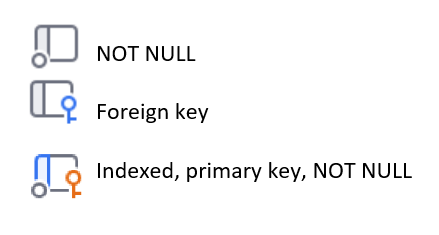
\includegraphics[width=\textwidth]{figures/ERLegend}
    \caption{Legende: ER-Diagramm}
    \label{fig:er-diagramm_legend}
\end{figure}

\begin{figure}[ht]
    \centering
    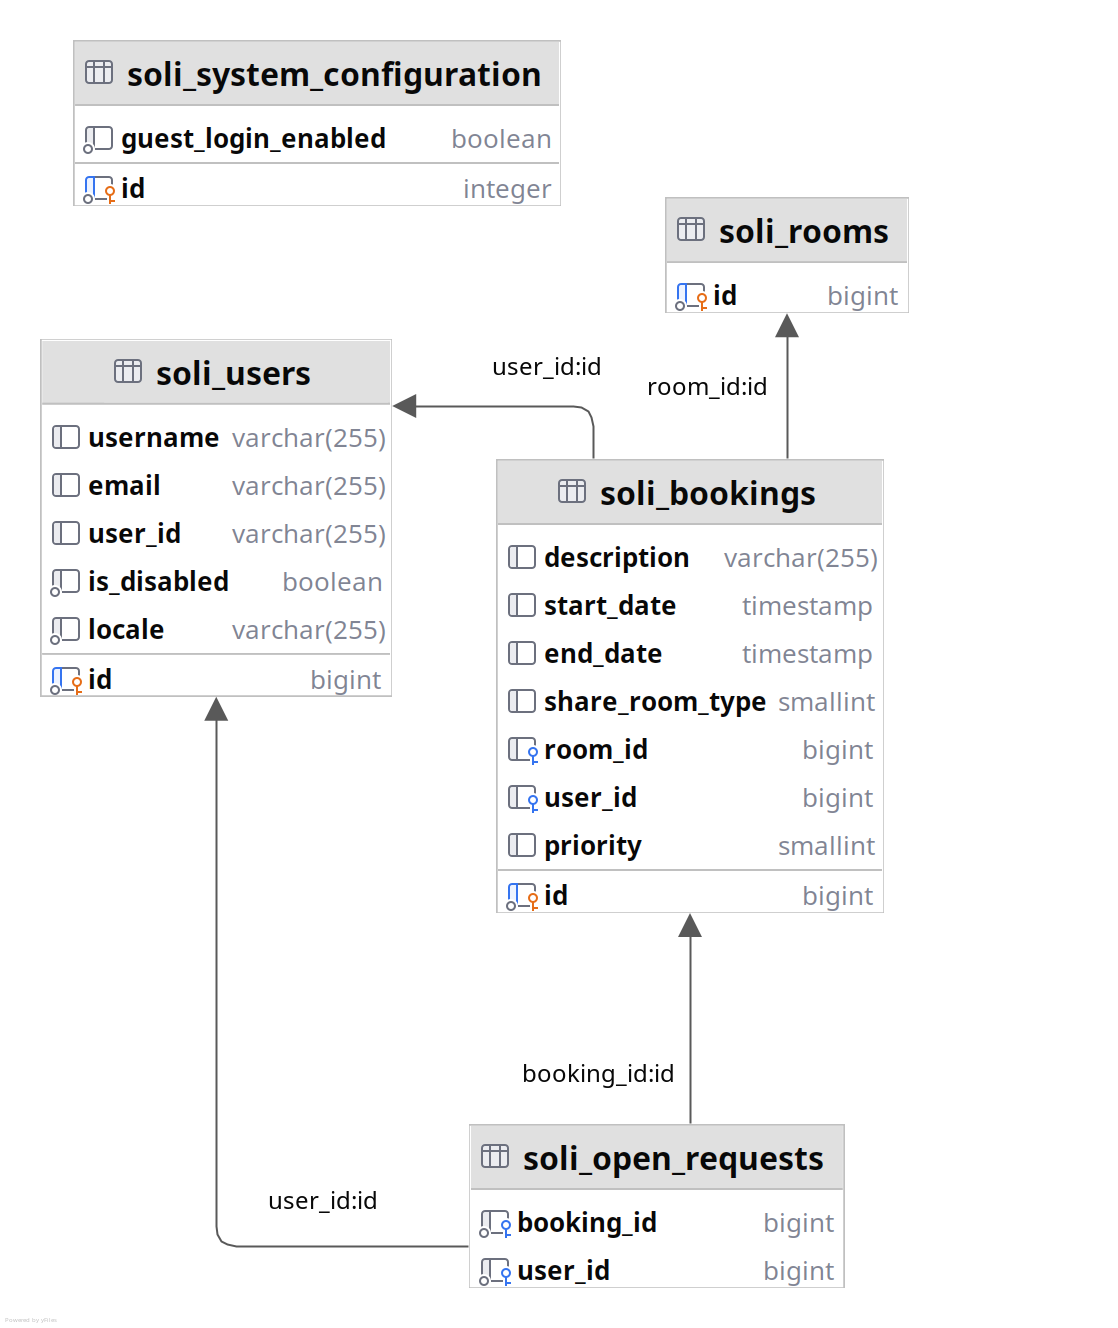
\includegraphics[width=\textwidth]{figures/database}
    \caption{ER-Diagramm}
    \label{fig:er-diagramm}
\end{figure}

\begin{figure}[ht]
    \centering
    
\includegraphics[width=\textwidth]{figures/impl-views/placeholder} % TODO add new ER-Diagramm (in lightmode pls)
    \caption{Neues ER-Diagramm}
    \label{fig:er-diagramm_new}
\end{figure}
%!TEX root = ../main.tex

\chapter{Tests und Coverage}
\label{ch:tests}

Für kontinuierliches Testen und zur Sicherstellung der Qualität des Codes wurden sowohl Unit- als auch Integrationstests geschrieben.
Diese werden nach jedem Push auf das Repository durch GitHub CI automatisiert ausgeführt.

Umgesetzt sind die Tests mit JUnit als Testframework, Mockito für Mocking und werden von Gradle gestartet.
Damit sichergestellt werden kann, dass die Tests in einem Realitätsnahen Umfeld laufen,
wird eine normale Postgres-Datenbank verwendet, welche in einem von Gradle gestarteten Docker-Container läuft.

Um die Abdeckung unseres Quellcodes durch die Tests sicherzustellen, setzen wir JaCoCo ein.
JaCoCo wird ebenfalls von Gradle gestartet und generiert nach jedem Testdurchlauf einen Report, der in GitHub CI angezeigt wird.
Bei einer zu niedrigen Testabdeckung wird zudem ein fehlgeschlagener Check in GitHub CI generiert.

Ausgenommen von den Tests ist lediglich der Inhalt des Pakets \textit{config},
da dieser lediglich der Konfiguration von Spring dient und nicht gut durch Unit- oder Integrationstests geprüft werden kann, sowie \textit{view} da dies schwer automatisiert visuell zu überprüfen.

\newpage

\section{Coverage}\label{sec:coverage}

Zum Ende der Implementationsphase haben wir in mehr als 150 Tests eine Coverage von 67\% erreicht.
Diese gliedert sich wie folgt in die verschiedenen Pakete auf:

\begin{table}[h]
    \centering
    \renewcommand{\arraystretch}{1.3}
    \begin{tabular}{l|c}
        \textbf{Paket} & \textbf{Line Coverage} \\
        \hline
        \hline
        \textit{Controller}  & 69\% \\
        \textit{Domain}      & 87\% \\
        \textit{DTO}         & 79\% \\
        \textit{Filter}      & 100\% \\
        \textit{Repository}  & 100\% \\
        \textit{Service}     & 84\% \\
        \hline
        \textit{Gesamt}      & 67\% \\
    \end{tabular}
    \caption{Coverage der verschiedenen Pakete}
    \label{tab:progress}
\end{table}

%!TEX root = ../main.tex

\chapter{Aktivität}
\label{chap:activity}

In Abbildung~\ref{fig:tasks} ist die Verteilung der Aufgaben unter unseren Teammitgliedern zu sehen.
Wie zu erkennen ist, wurde mit einzelnen Ausnahmen jedem Teammitglied für jede Woche eine Aufgabe zugeteilt.
Da wir vermuteten, dass die Umsetzung der Öffnungszeitenfunktion überdurchschnittlich kompliziert sein könnte,
entschieden wir uns, dieser Funktion zwei Wochen zuzuweisen.

Die im Diagramm dargestellte Zeitaufteilung wurde nahezu vollständig eingehalten,
die Zeitschätzungen bei der Aufteilung der Funktionen scheint dem tatsächlichen Aufwand also sehr nahe gewesen zu sein.

\begin{figure}[ht]
    \centering
    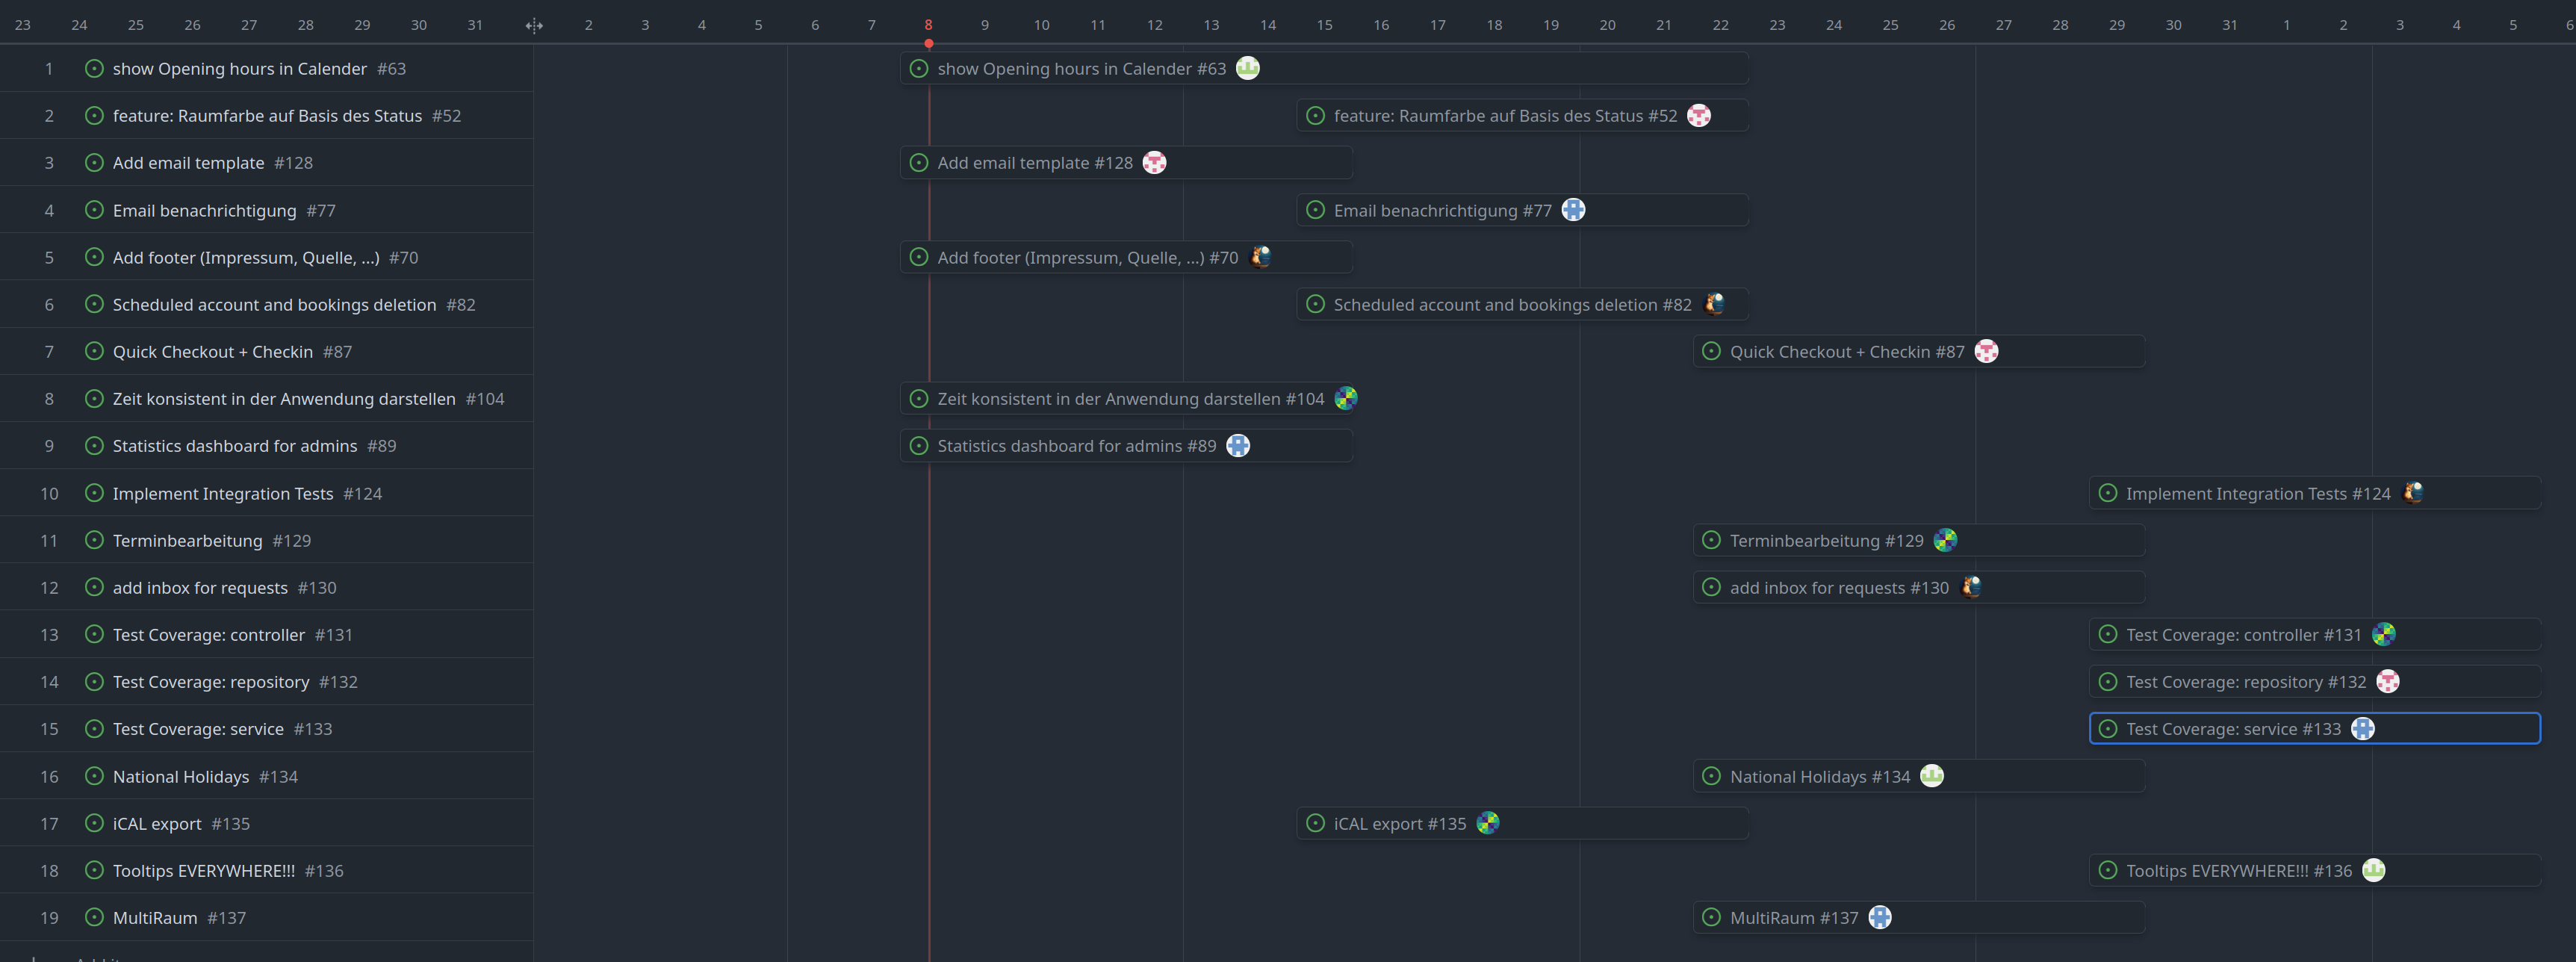
\includegraphics[width=\textwidth]{figures/tasks}
    \caption{Verteilung der Aufgaben}
    \label{fig:tasks}
\end{figure}

In Abbildung~\ref{fig:commits} ist die Verteilung der Commits pro Stunde und Wochentag dargestellt.
In dieser ist zu erkennen, dass die Entwicklung der Anwendung größtenteils in den üblichen Arbeitszeiten von 9 bis 17 Uhr verlief.
Während an Wochenenden und Feiertagen einzelne Commits vorkommen, sind diese in der Regel auf kleinere Änderungen beschränkt.
Für die Planung des Projekts ist dies ein klarer Erfolg, da die Aufgaben offenbar gut über die Zeit verteilt werden konnten.

\begin{figure}[ht]
    \centering
    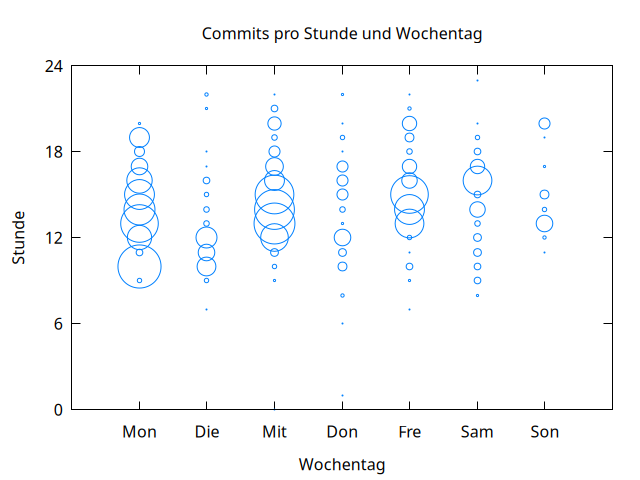
\includegraphics[width=\textwidth]{figures/hours}
    \caption{Commits pro Stunde und Wochentag}
    \label{fig:commits}
\end{figure}
%!TEX root = ../main.tex

\chapter{View}
\label{chap:view}


\section{Haupseite und Buchung}

Das Mockup der Startseite der Anwendung ist in \ref{fig:startseite} dargestellt.

Die entsprechende implementierte Startseite wird gezeigt in \ref{fig:impl-startseite}.

\begin{figure}[ht]
    \centering
    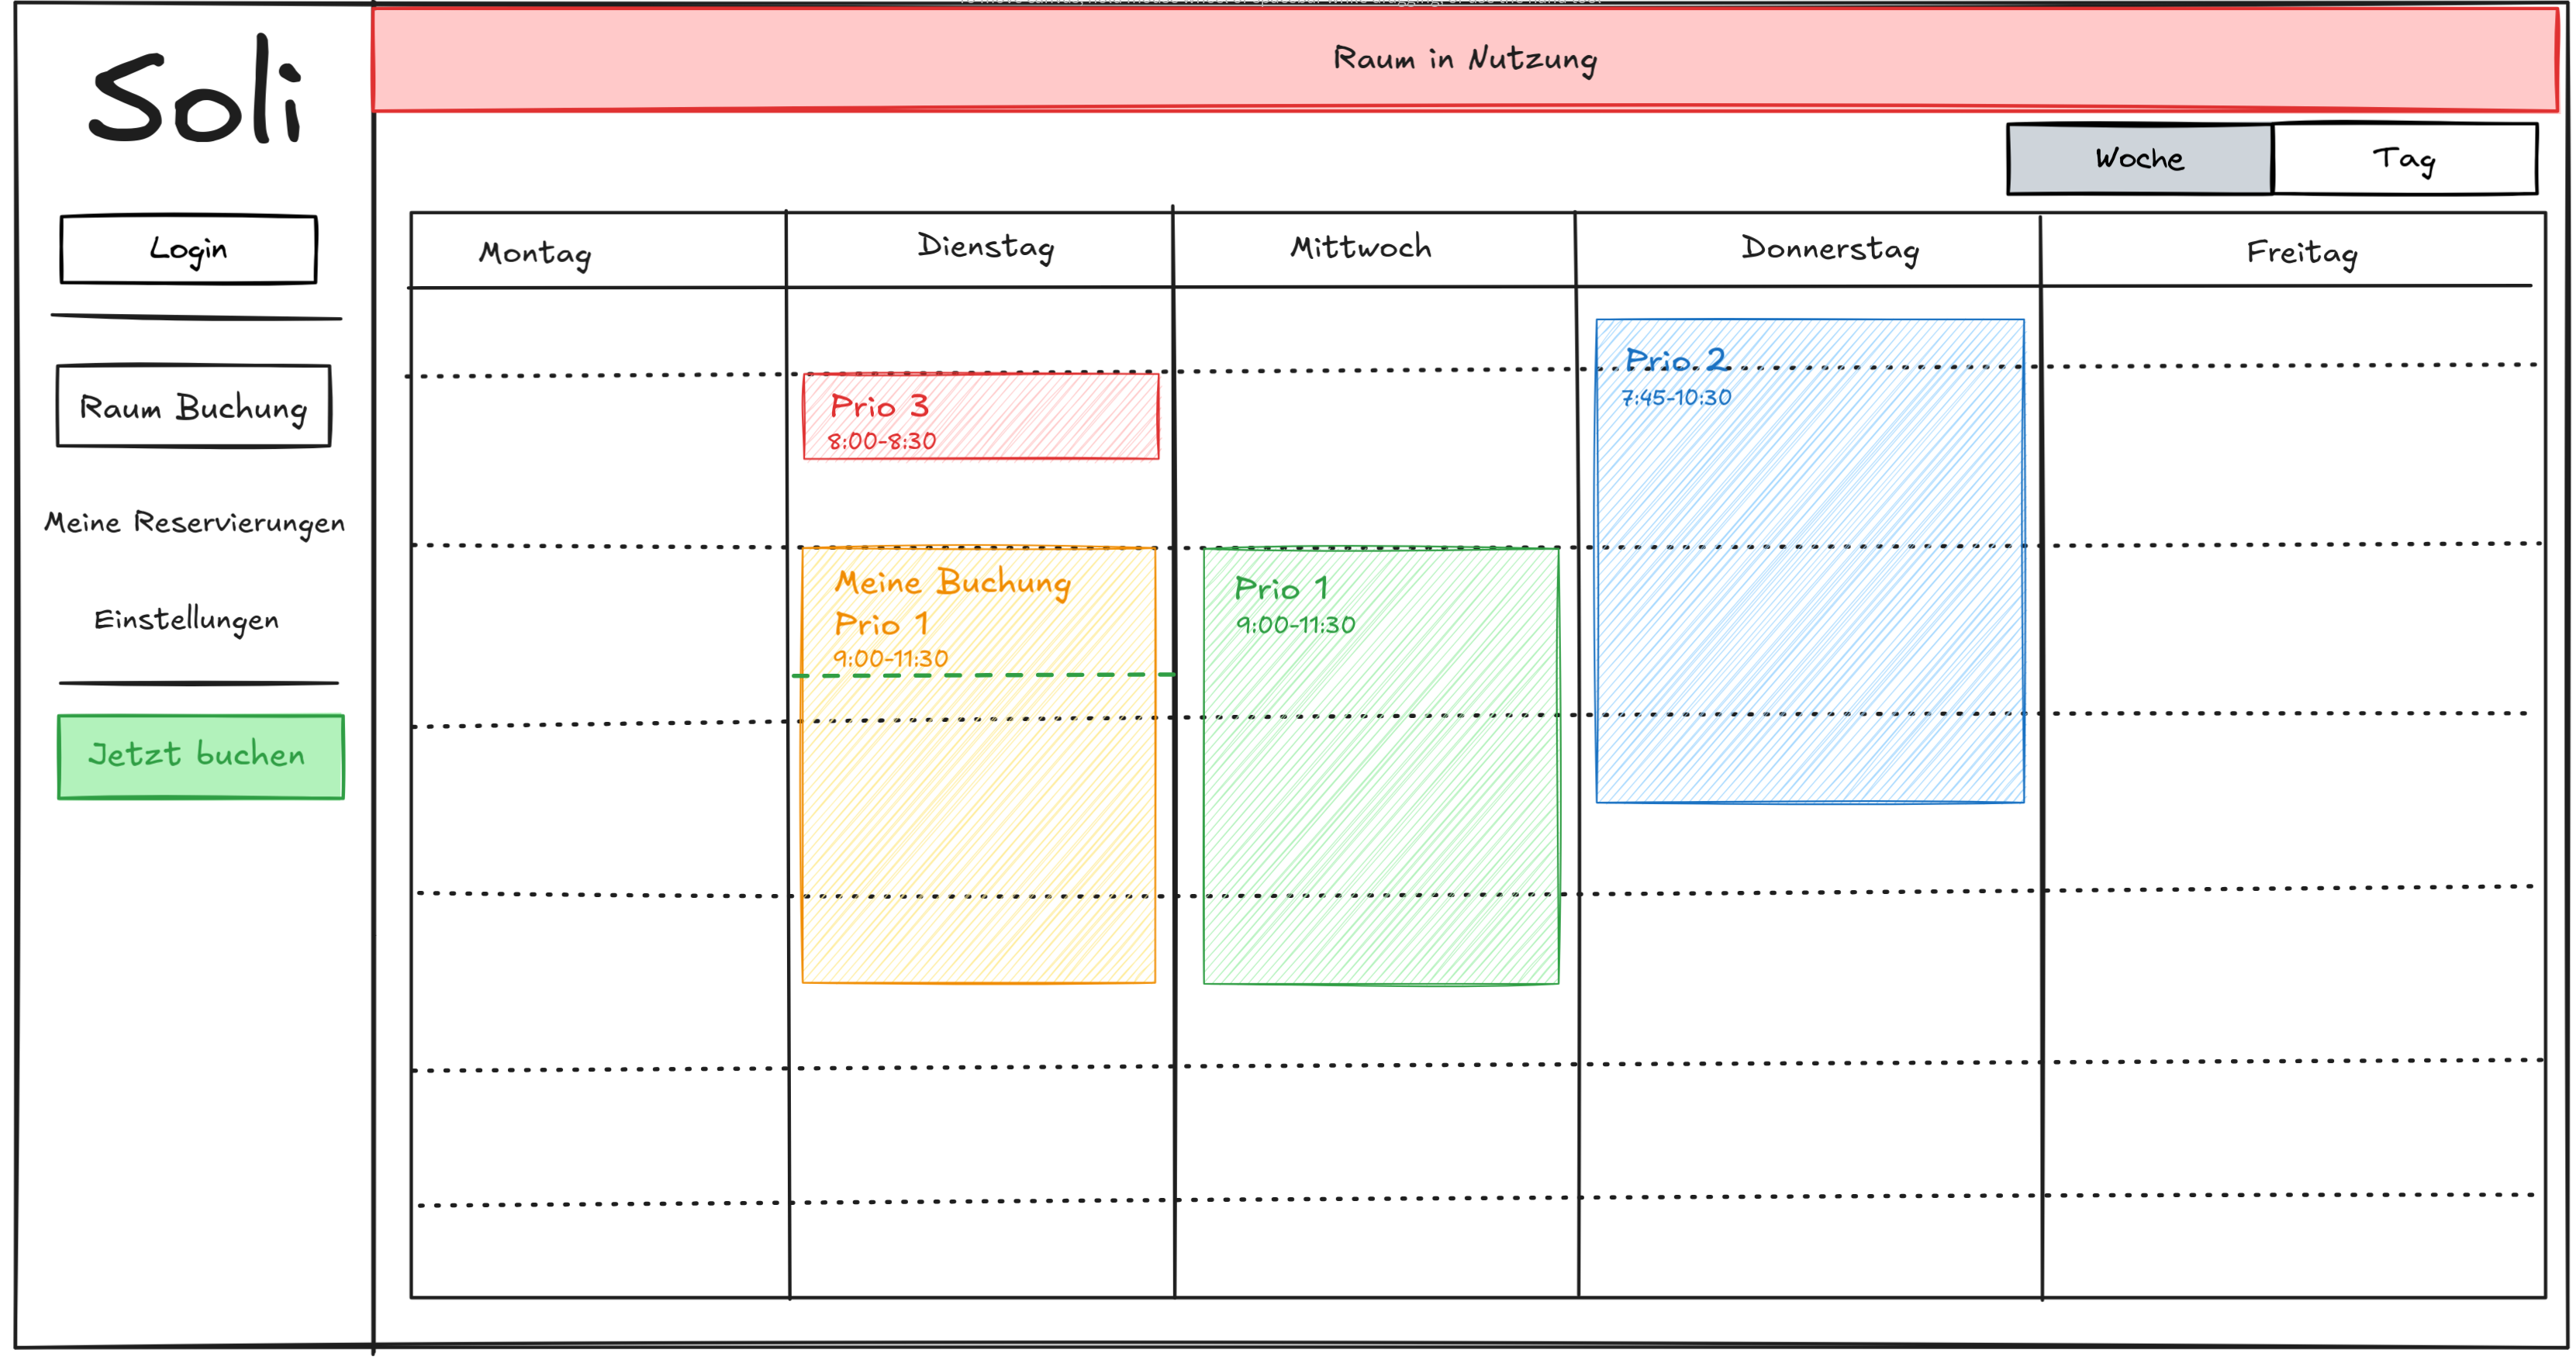
\includegraphics[width=\textwidth]{figures/mockup/startseite}
    \caption{Startseite der Anwendung}
    \label{fig:startseite}
\end{figure}
\pagebreak

\begin{figure}[ht]
    \centering
    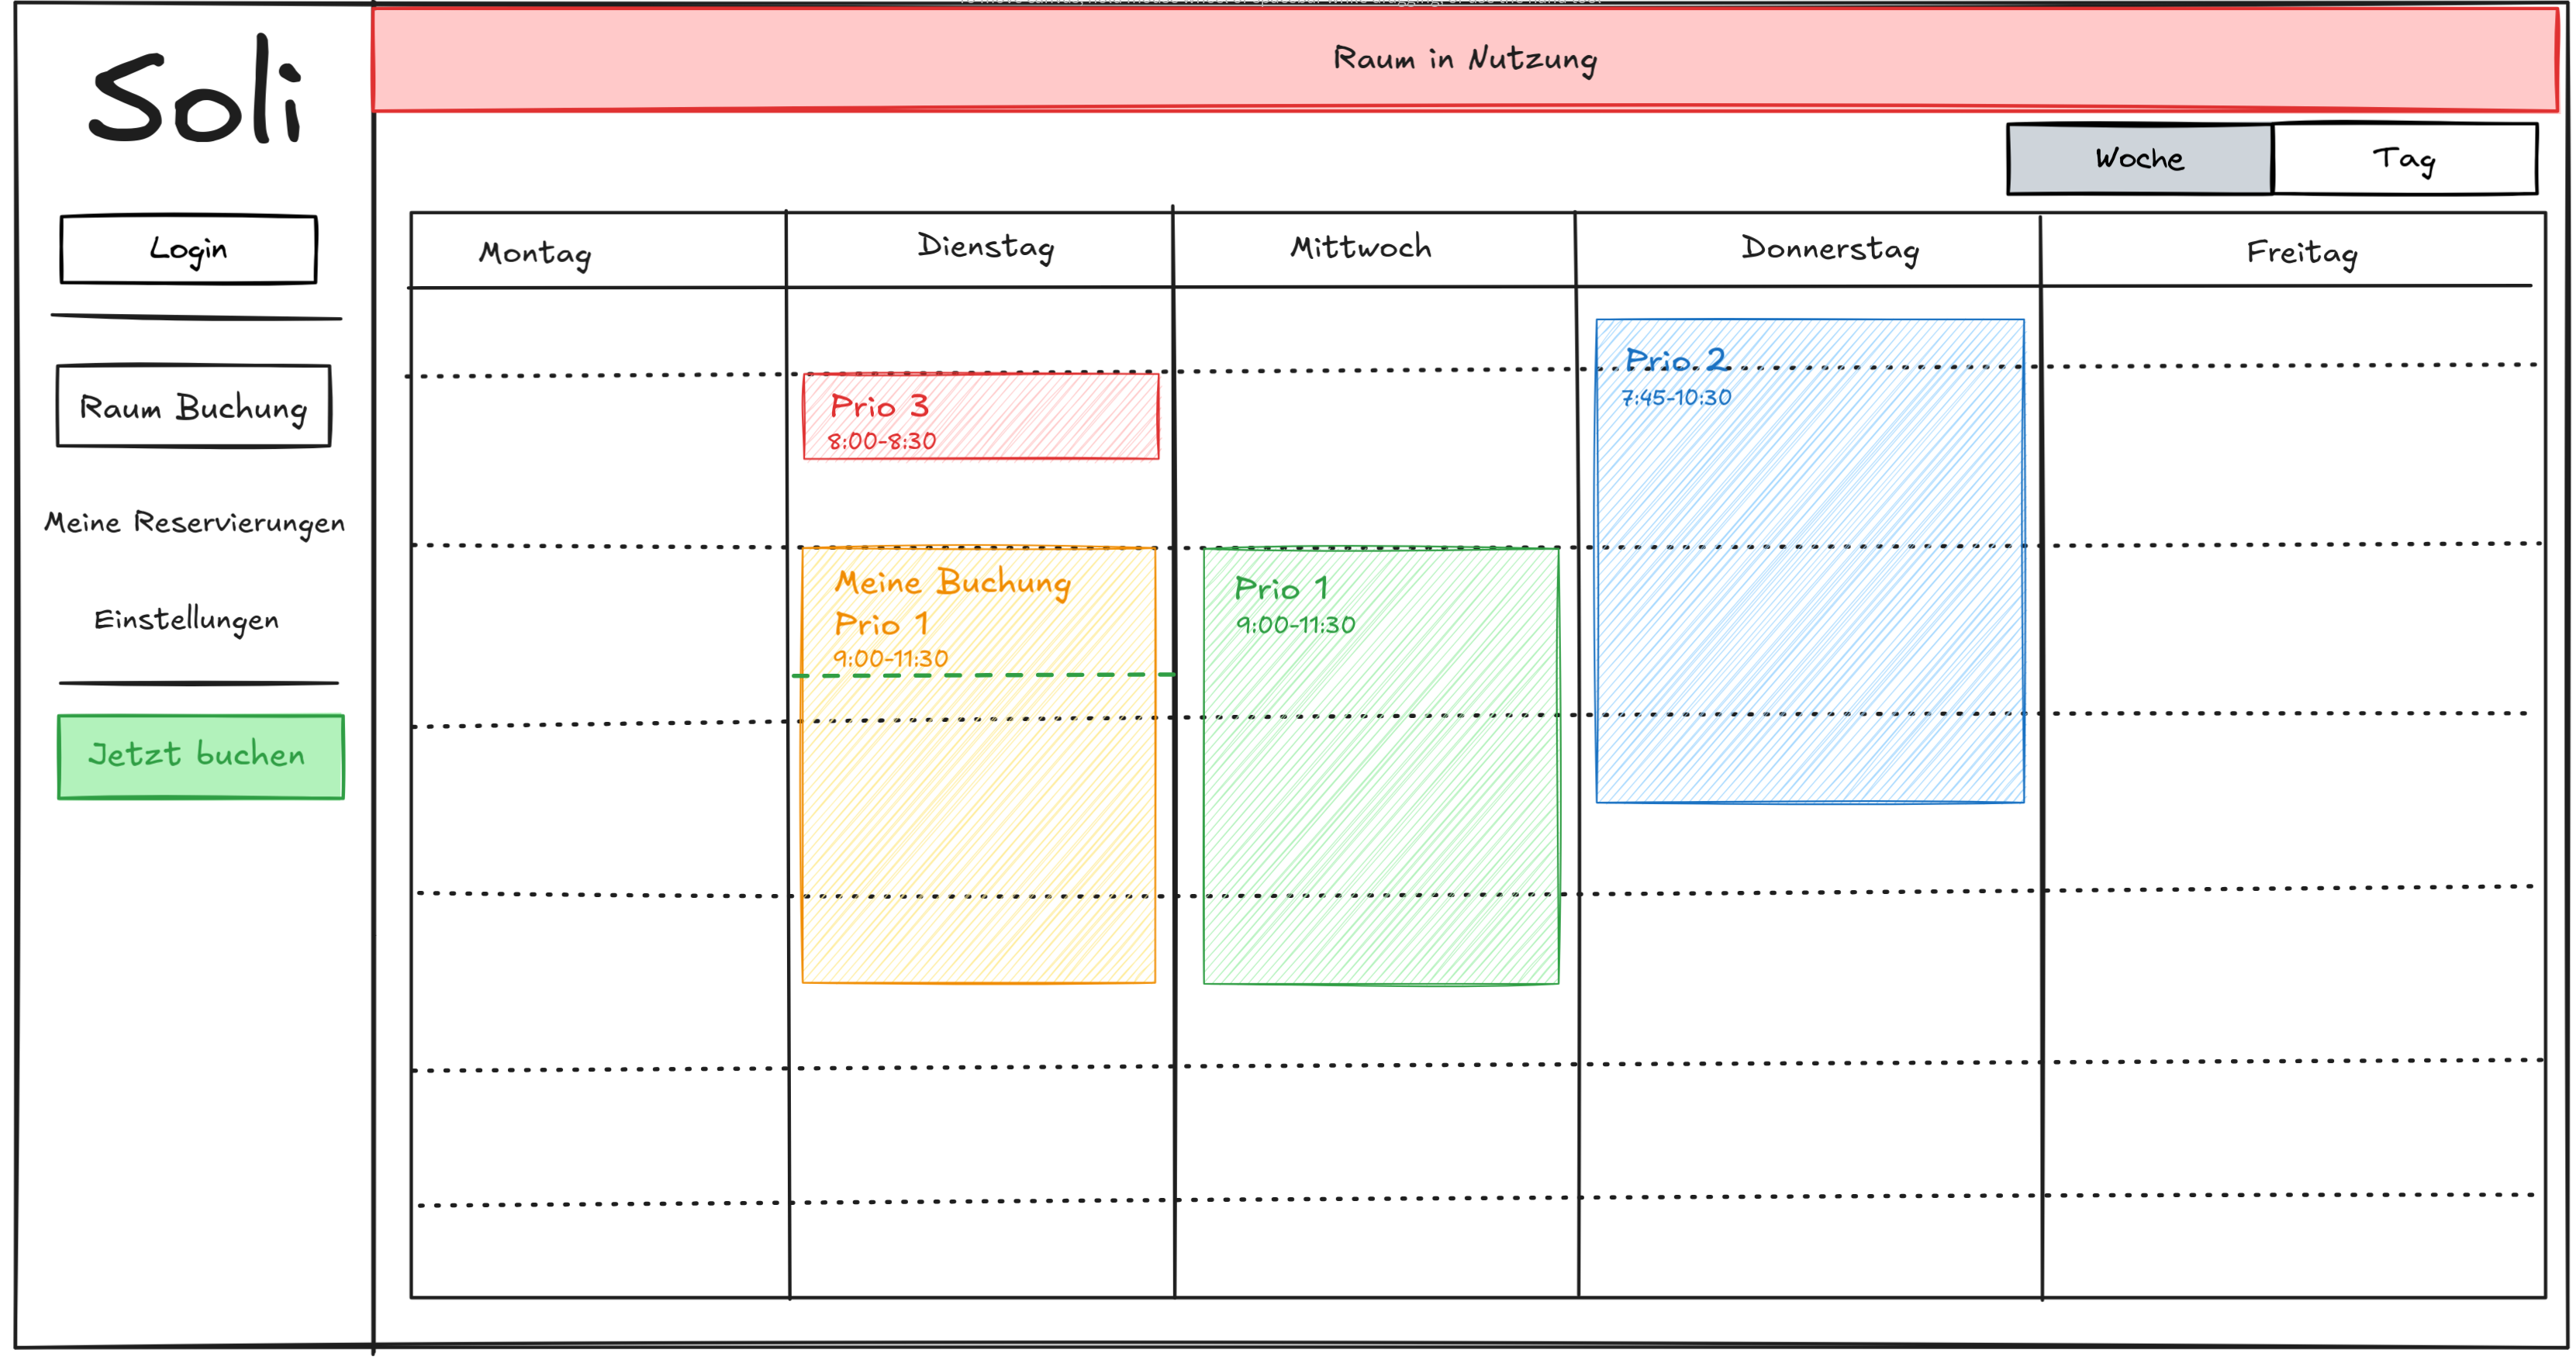
\includegraphics[width=\textwidth]{figures/mockup/startseite}
    \caption{Implentierung: Startseite der Anwendung}
    \label{fig:impl-startseite}
\end{figure}
\pagebreak

Sollten Nutzende eine Buchung vornehmen wollen, so klicken diese in den gewünschten Zeitraum
und es wird der Dialog in \ref{fig:buchung} dargestellt.

Der Dialog bietet Nutzenden die Möglichkeit, den genauen Start- und Endzeitpunkt des Termins festzulegen.

Außerdem können Nutzende die Priorität des Termins in Form einer Zahl zwischen 1 und 3 festlegen.
Nutzende können auch angeben, ob sie bereit sind, den Raum mit anderen Nutzenden zu teilen.
Für diesen Zweck werden Ihnen drei Optionen bereitgestellt: \textit{Ja}, \textit{Nein} und \textit{Auf Anfrage}.
Siehe dazu auch \ref{fig:buchung}.

Letztlich können Nutzende eine Beschreibung für den Termin hinterlegen, die anderen angemeldeten Nutzenden angezeigt wird.

\begin{figure}[ht]
    \centering
    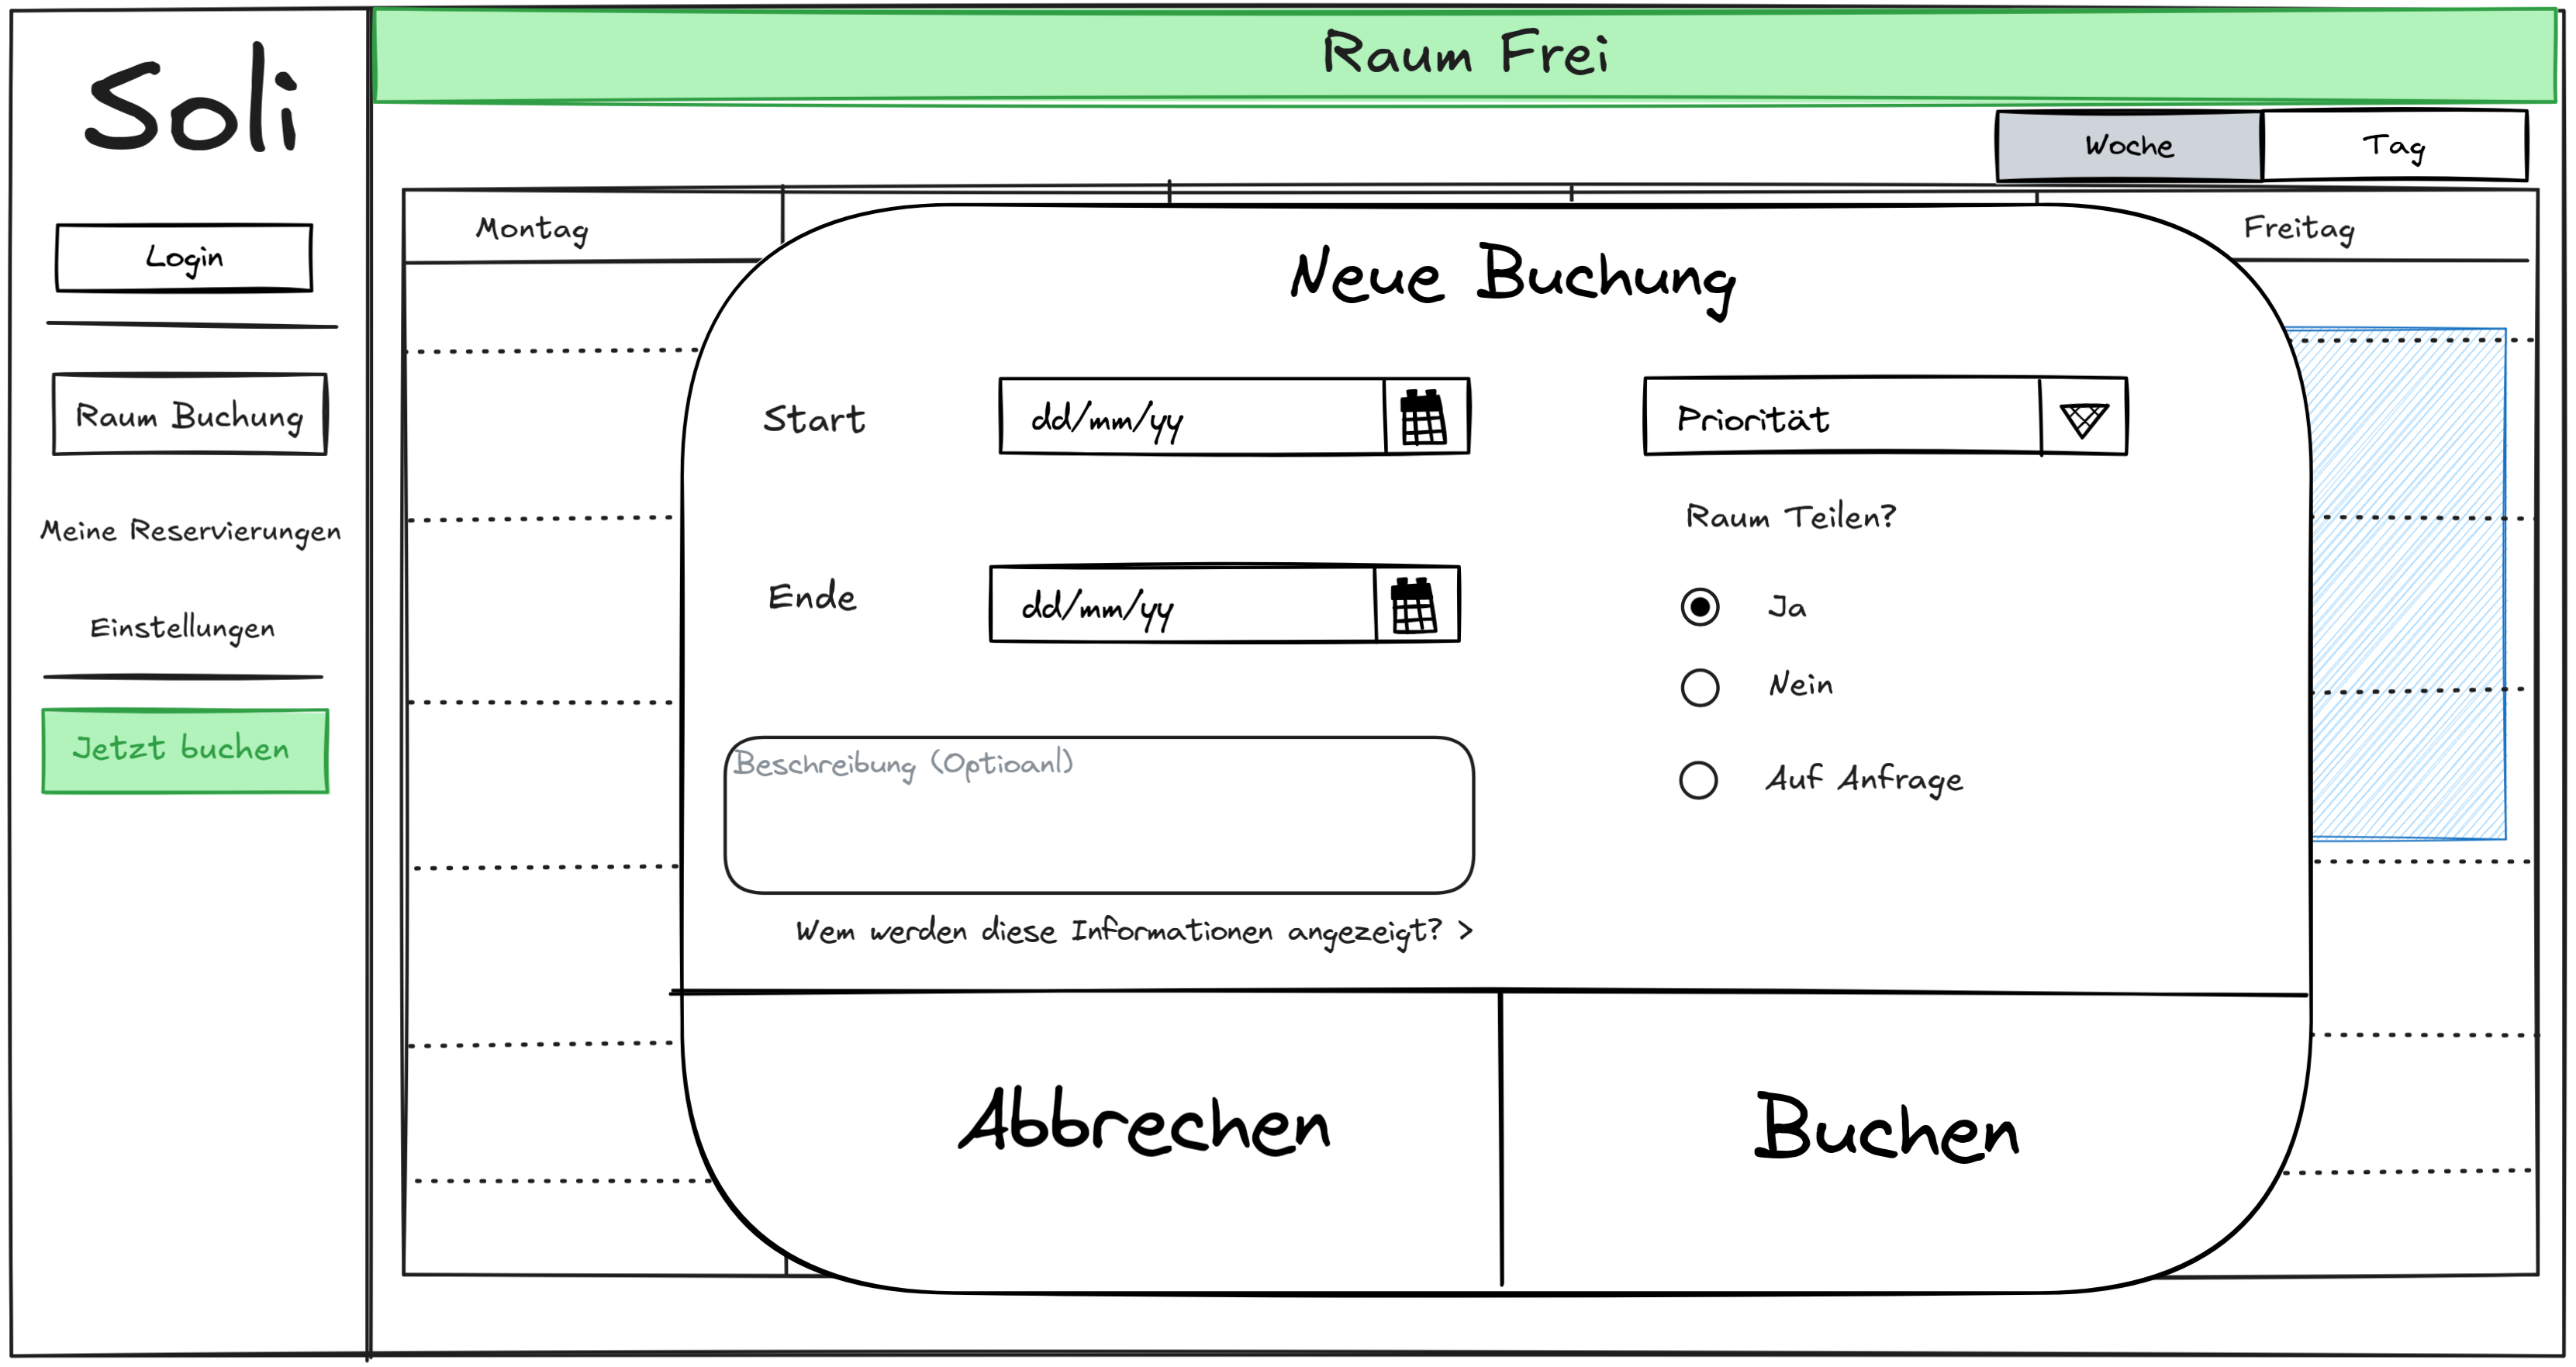
\includegraphics[width=\textwidth]{figures/mockup/buchungsdialog} % TODO Change this link to correct impl pic
    \caption{Termin-erstellen}
    \label{fig:buchung}
\end{figure}
\clearpage

In \ref{fig:login} ist die Anmeldungsansicht dargestellt und in \ref{fig:impl-login} ist die tatsächliche Implementierung zu sehen.

\begin{figure}[ht]
    \centering
    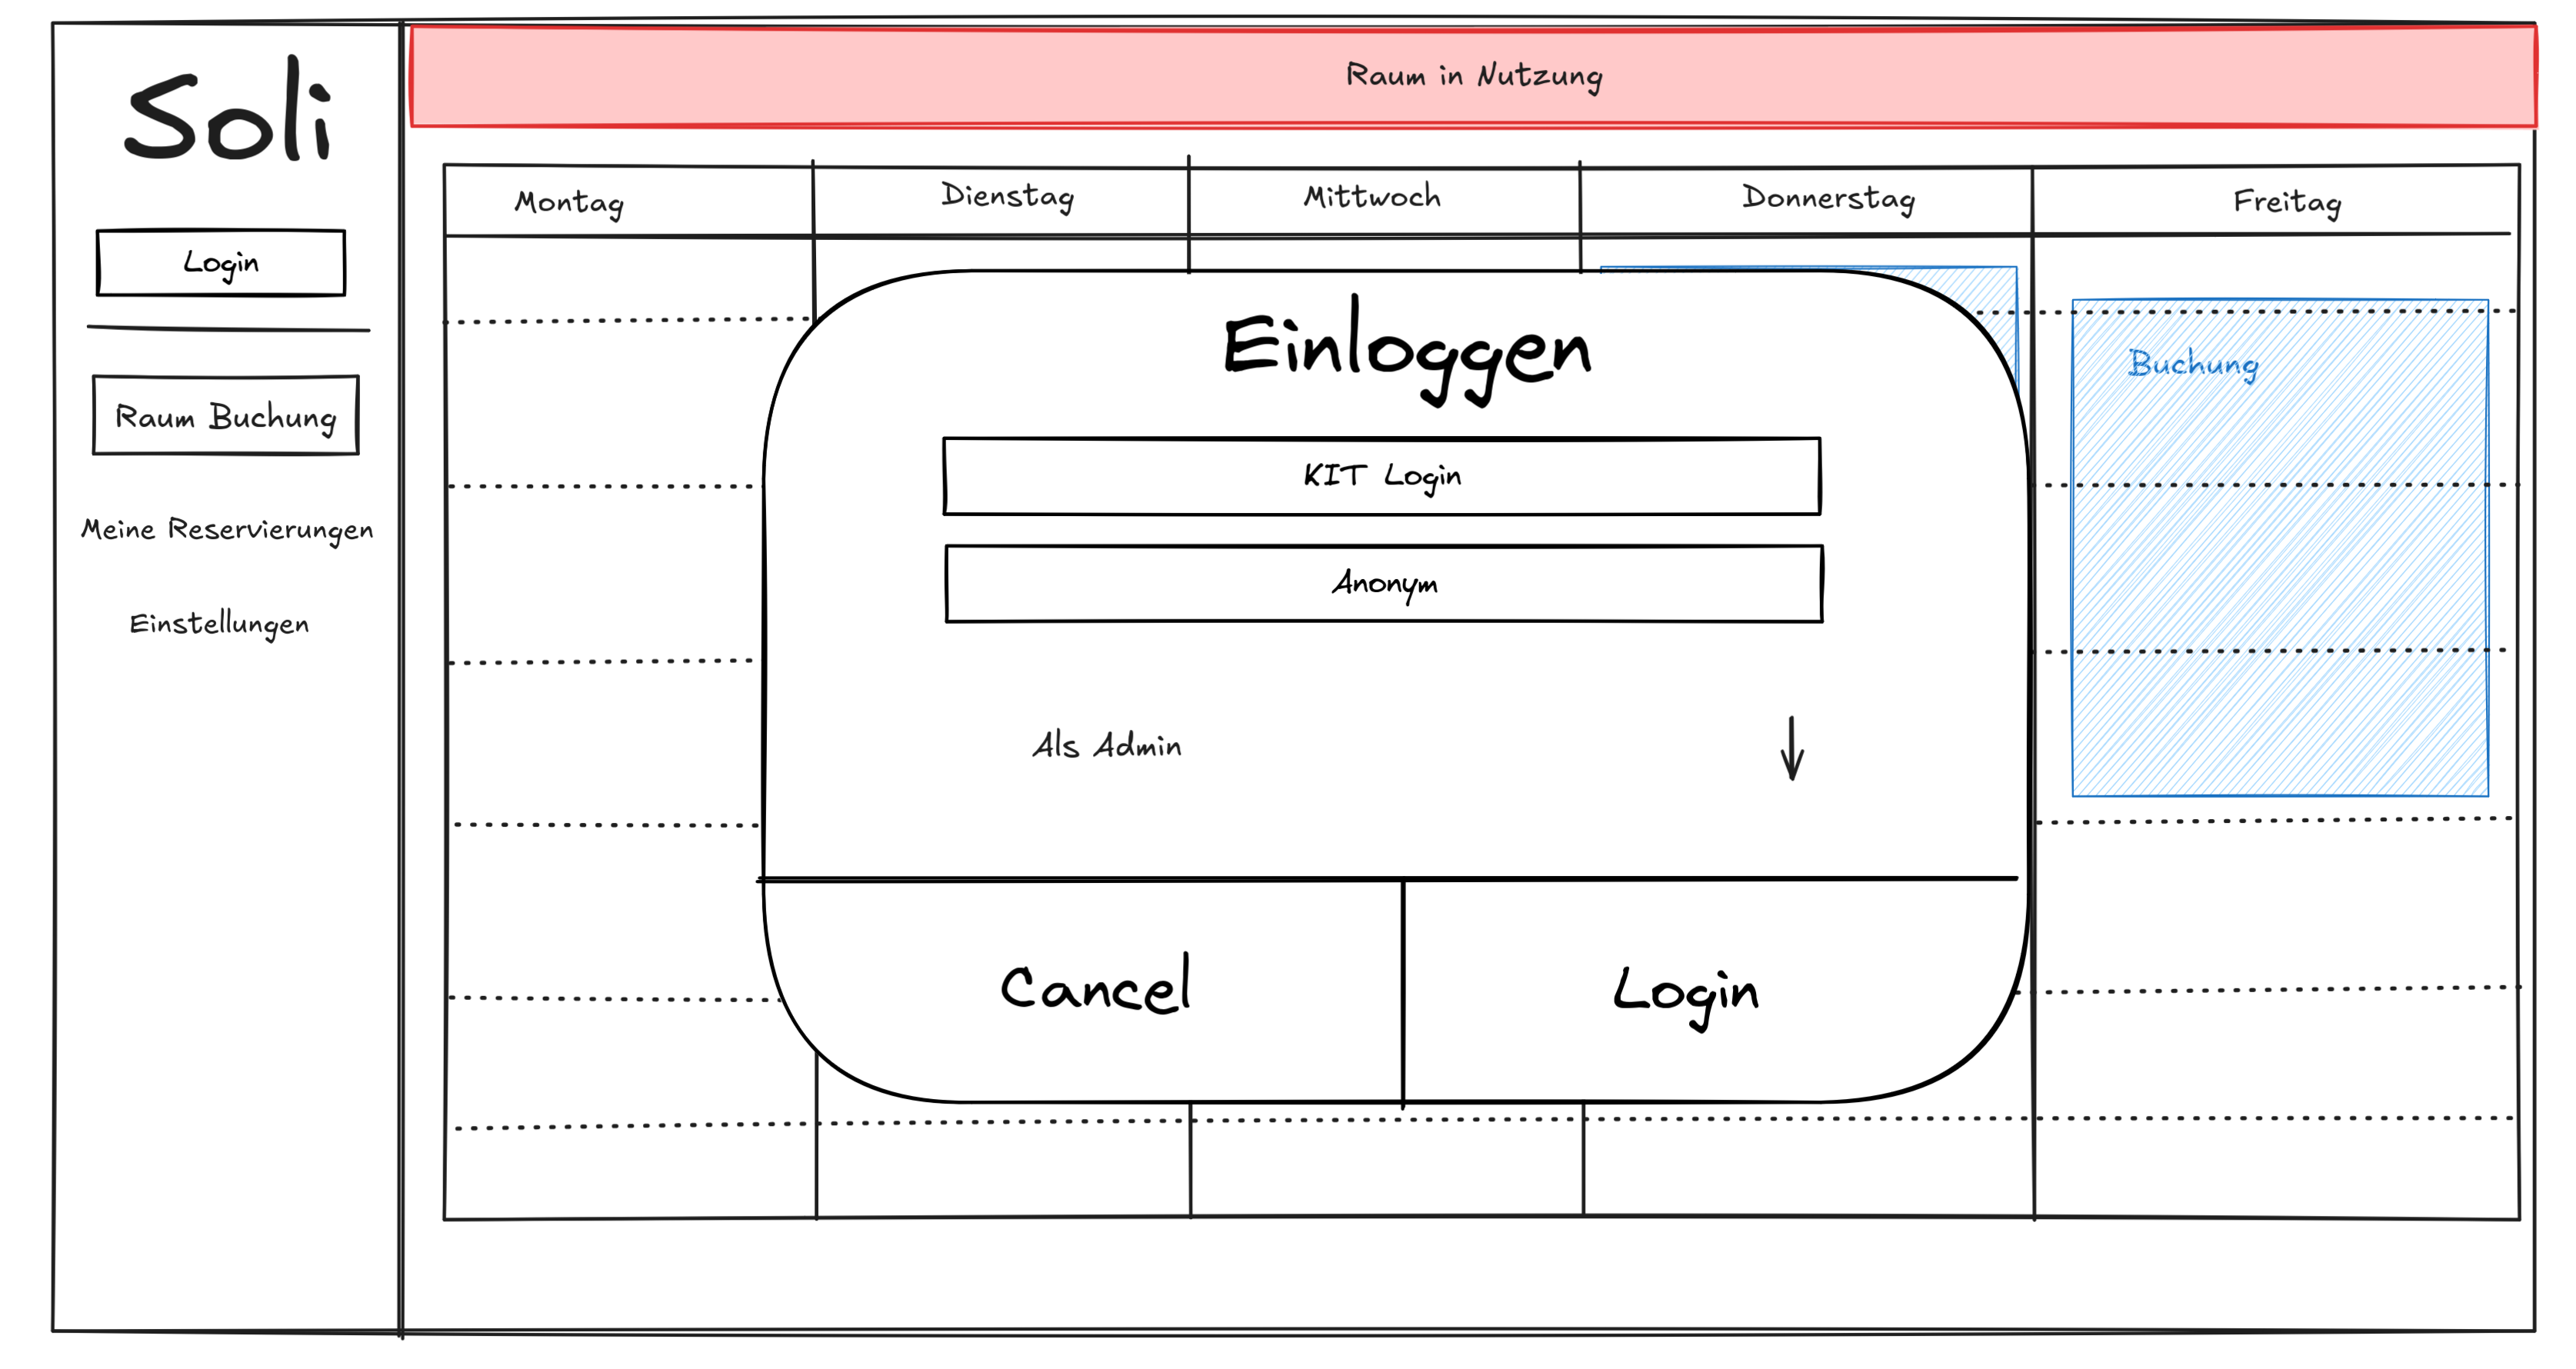
\includegraphics[width=\textwidth]{figures/mockup/anmeldungsseite}
    \caption{Anmeldungsseite}
    \label{fig:login}
\end{figure}
\clearpage

\begin{figure}[ht]
    \centering
    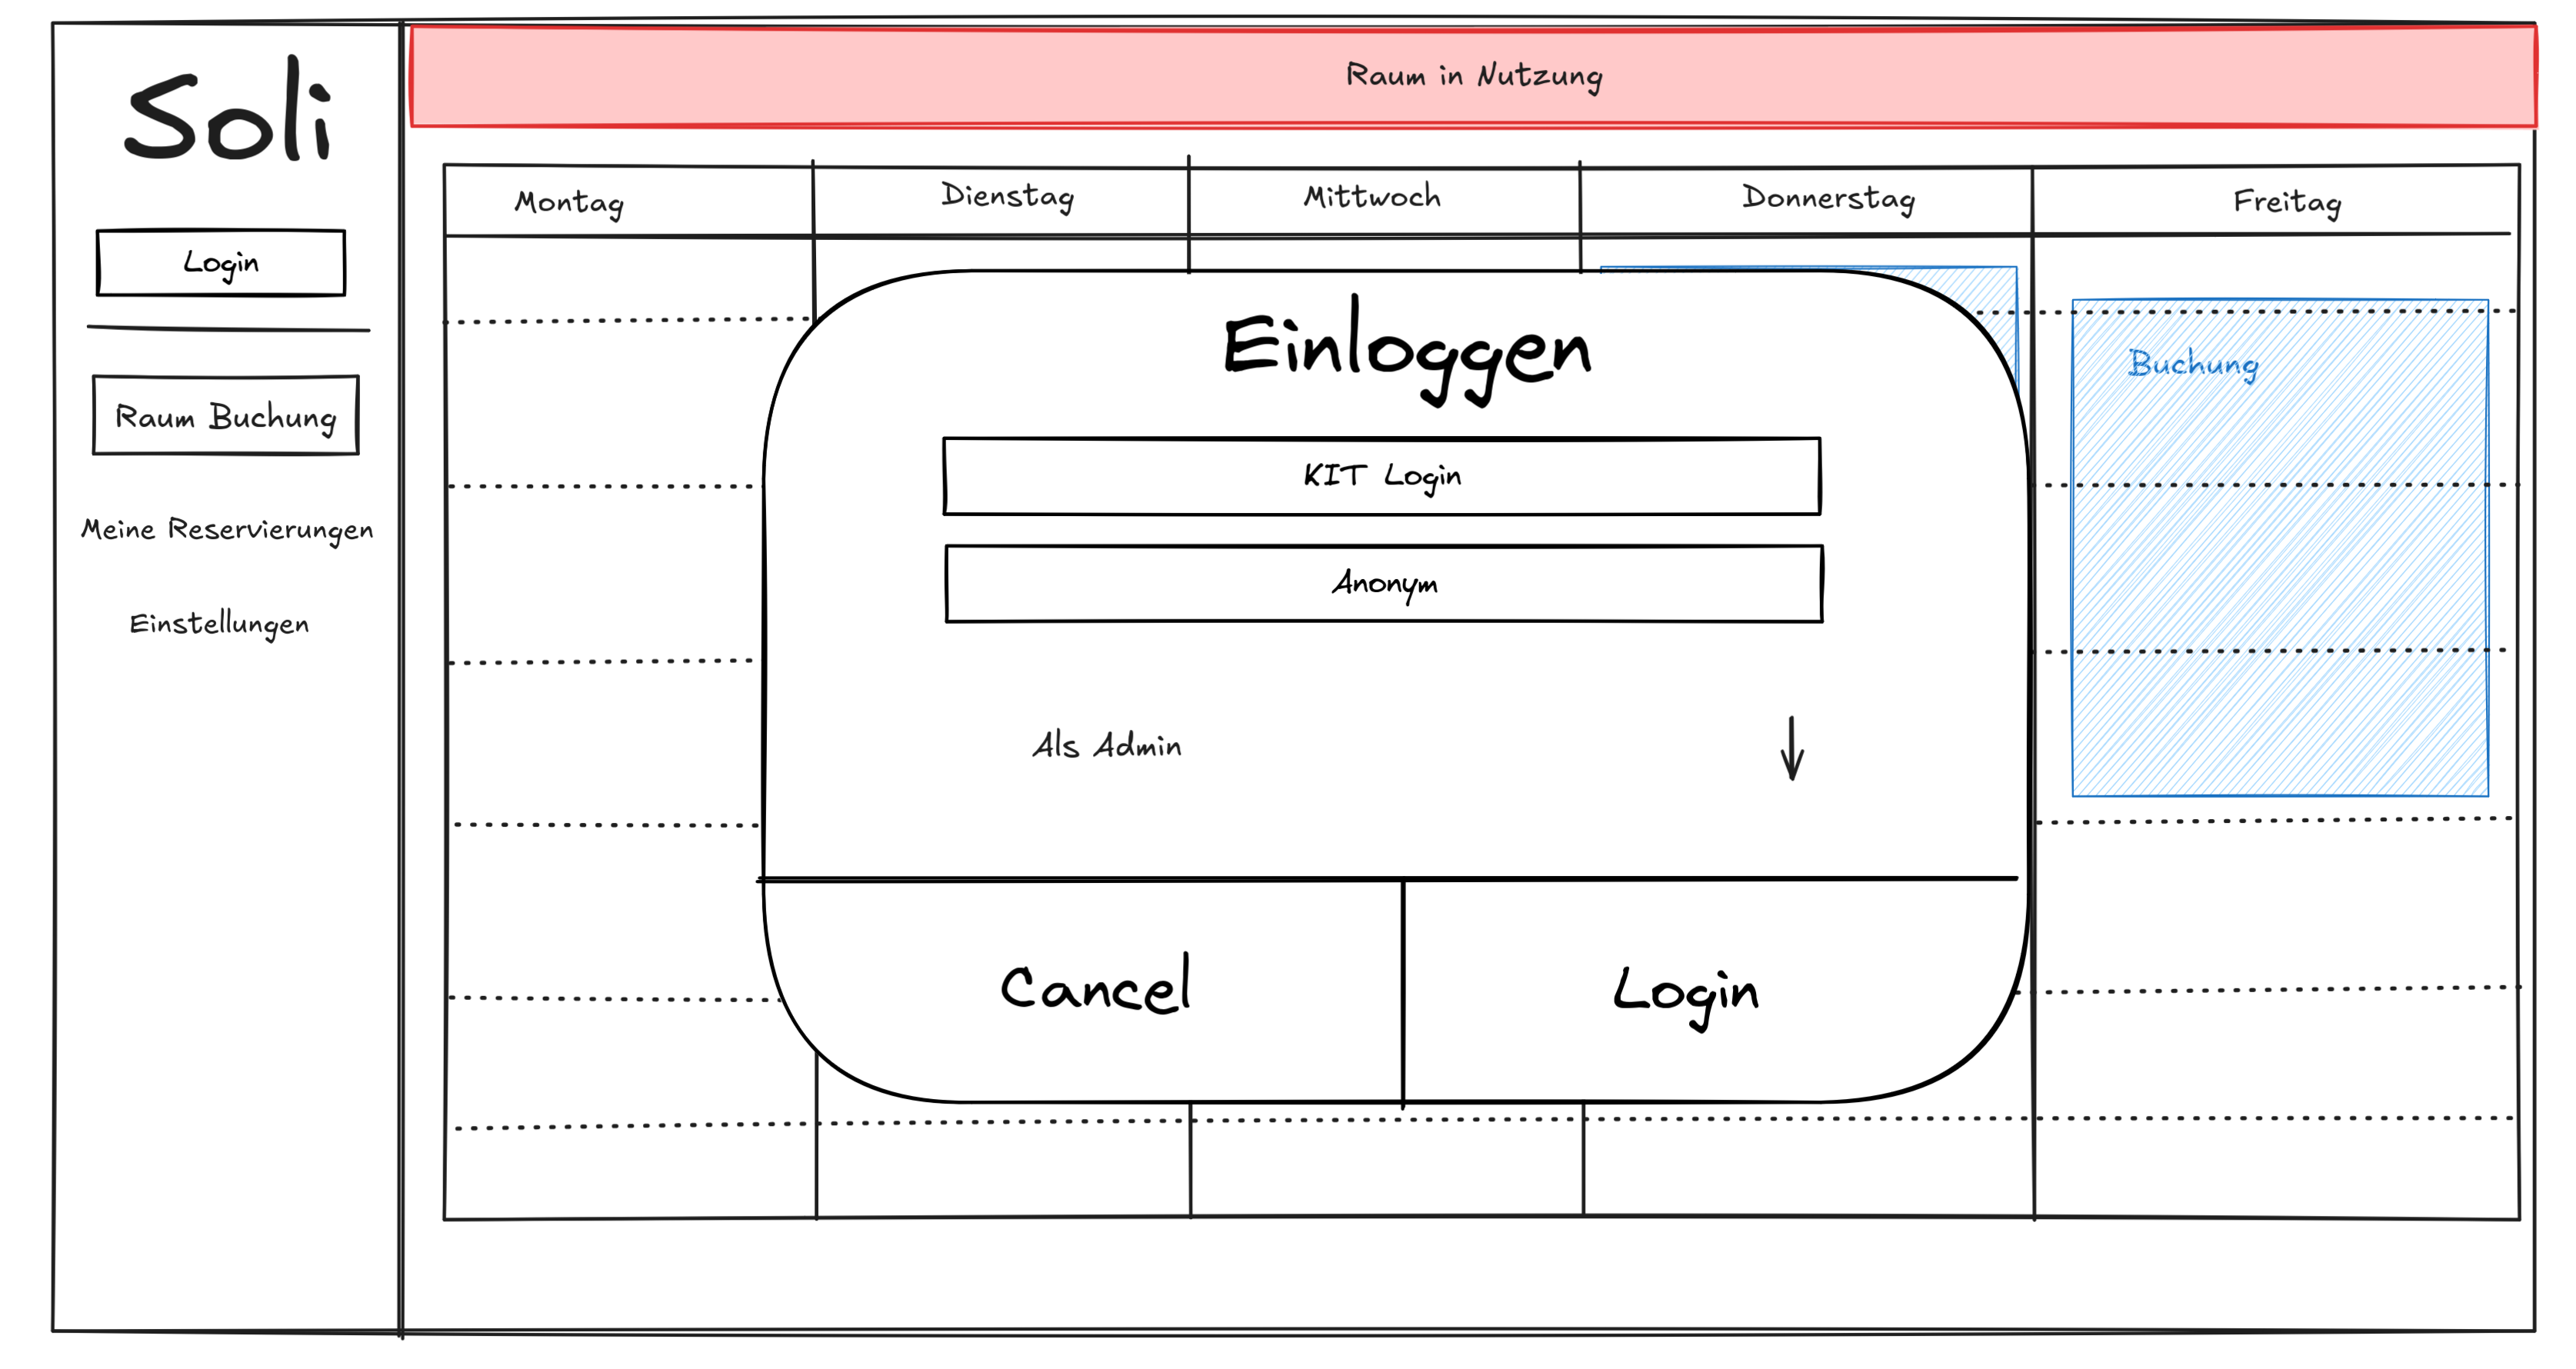
\includegraphics[width=\textwidth]{figures/mockup/anmeldungsseite} % TODO Change this link to correct impl pic
    \caption{Implementierung: Anmeldungsseite}
    \label{fig:impl-login}
\end{figure}
\clearpage

Sind Nutzende eingeloggt und belegen den Raum,
so wird ihnen die in Abbildung \ref{fig:checkout} dargestellte Ansicht angezeigt.
Hier können Nutzende den Raum wieder über den Quick-Checkout-Button freigeben.

Die Implementierung davon ist in \ref{fig:impl-checkout} zu sehen.


Ziel dieser Ansicht ist es, Nutzenden das frühe Freigeben des Raumes ohne unnötigen Mehraufwand zu ermöglichen.
\begin{figure}[ht]
    \centering
    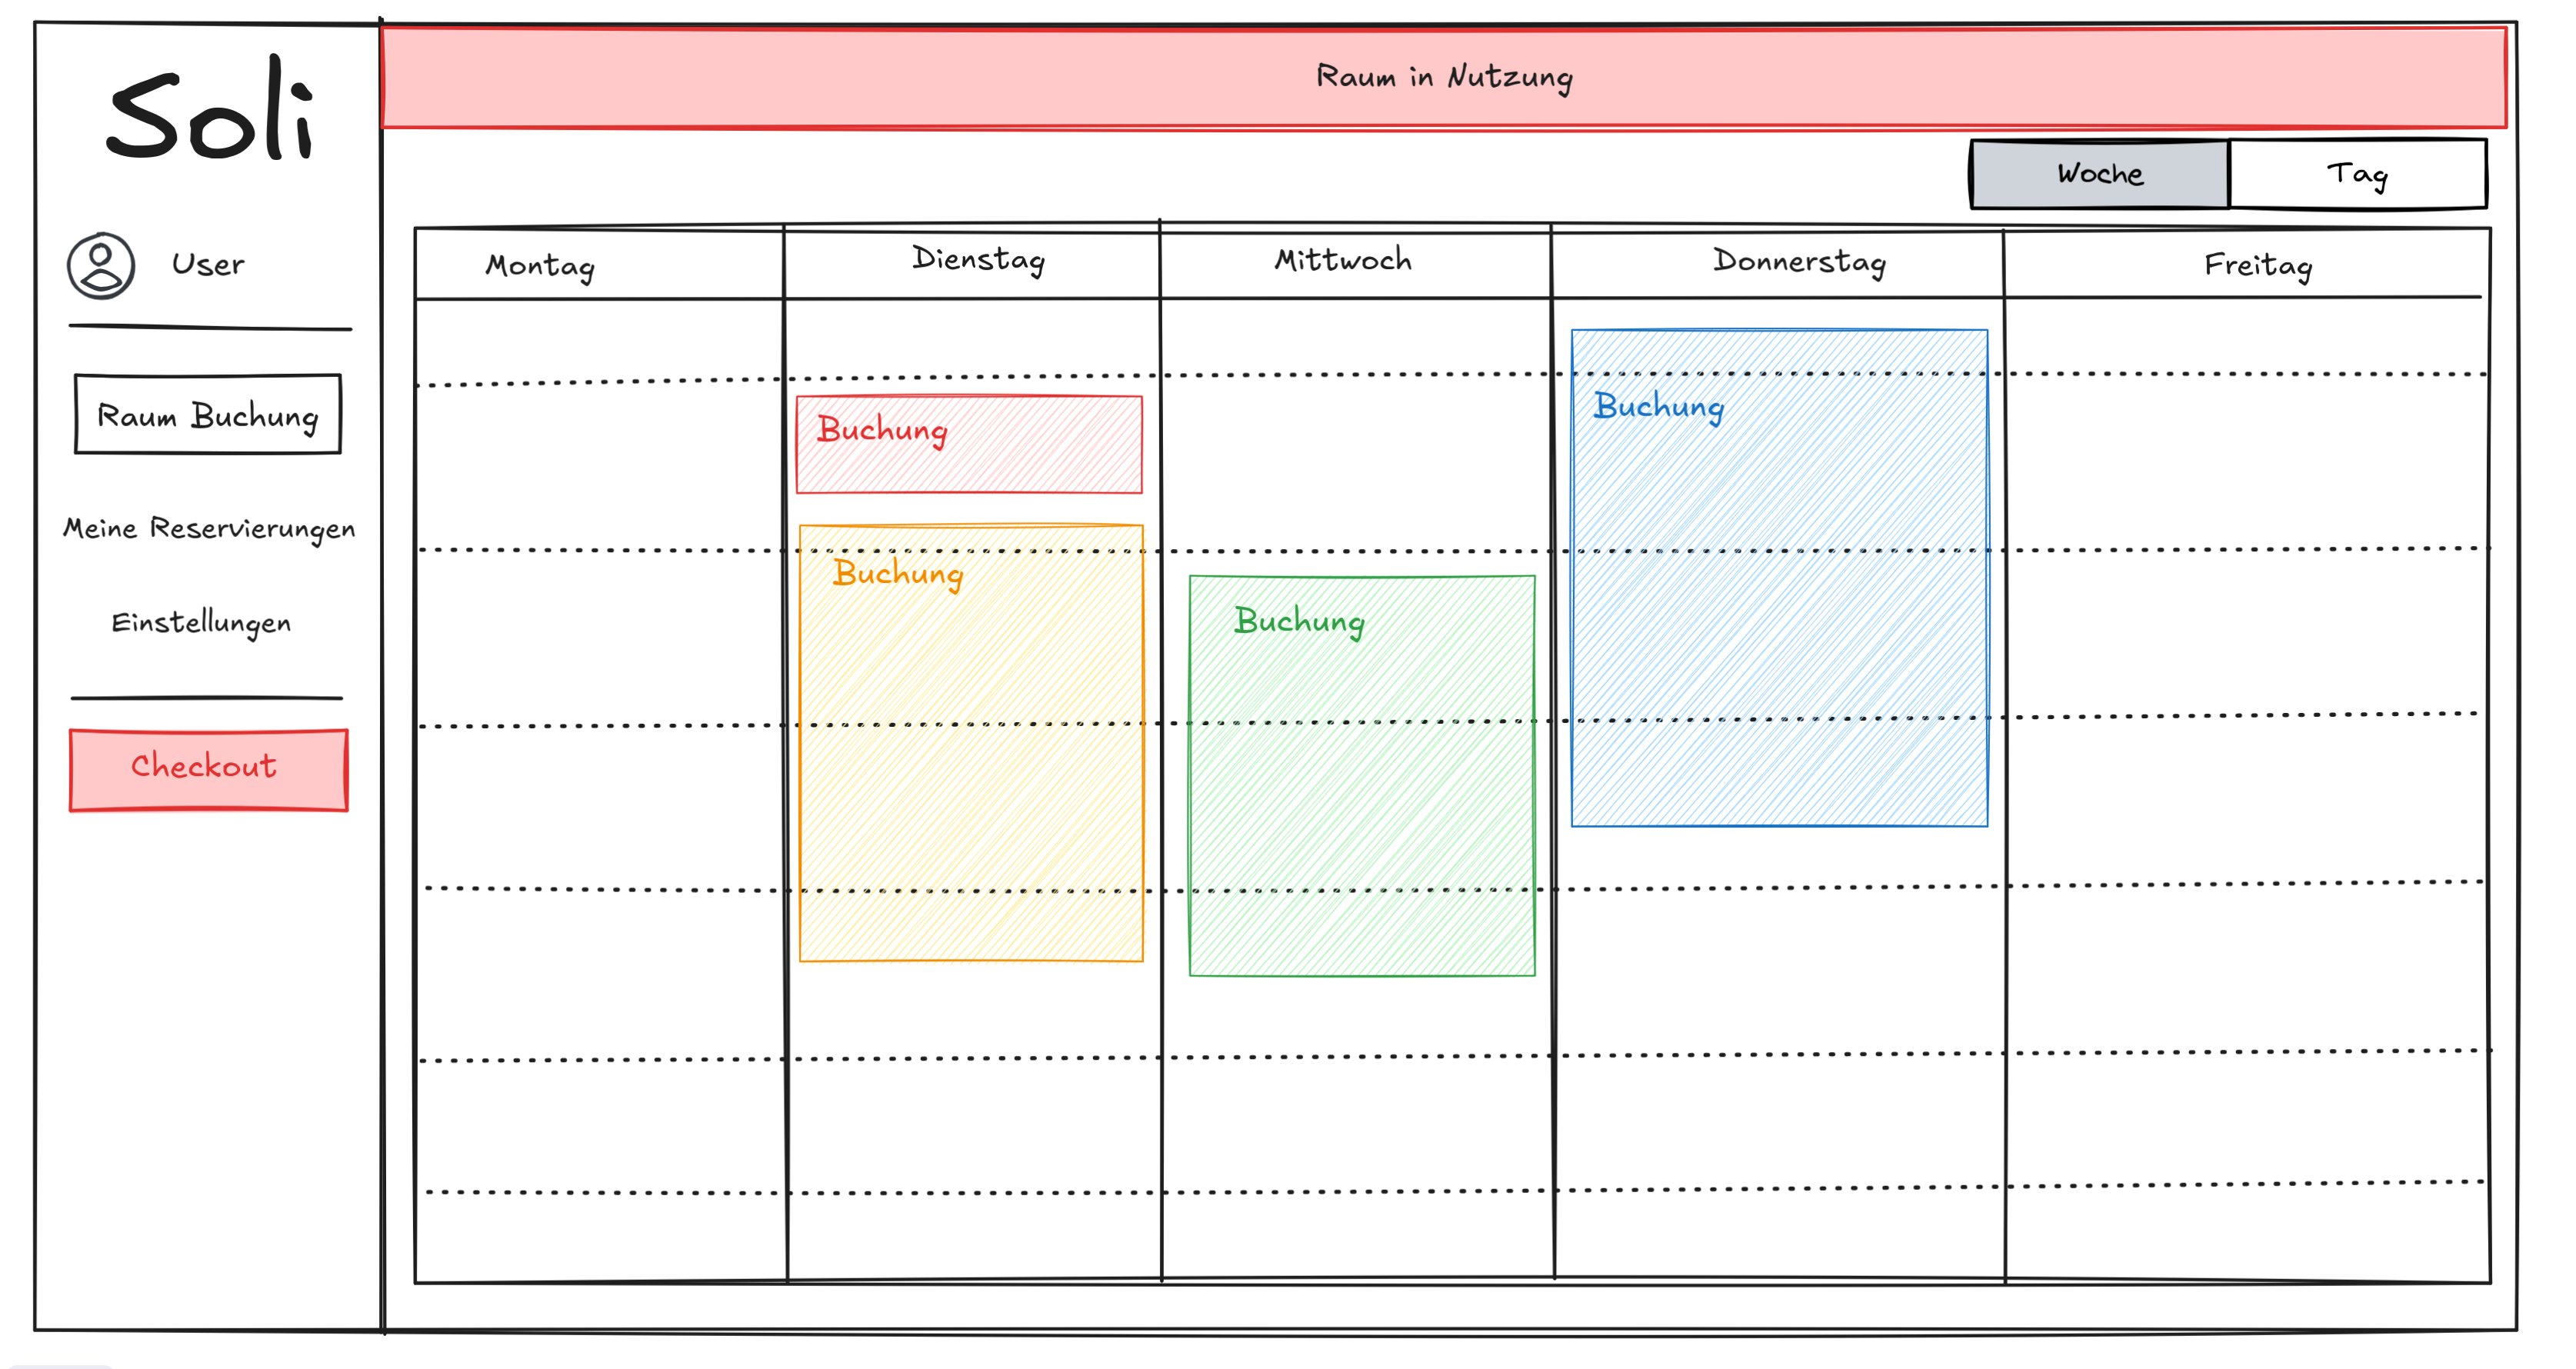
\includegraphics[width=\textwidth]{figures/mockup/checkout}
    \caption{Quick Checkout}
    \label{fig:checkout}
\end{figure}
\clearpage

\begin{figure}[ht]
    \centering
    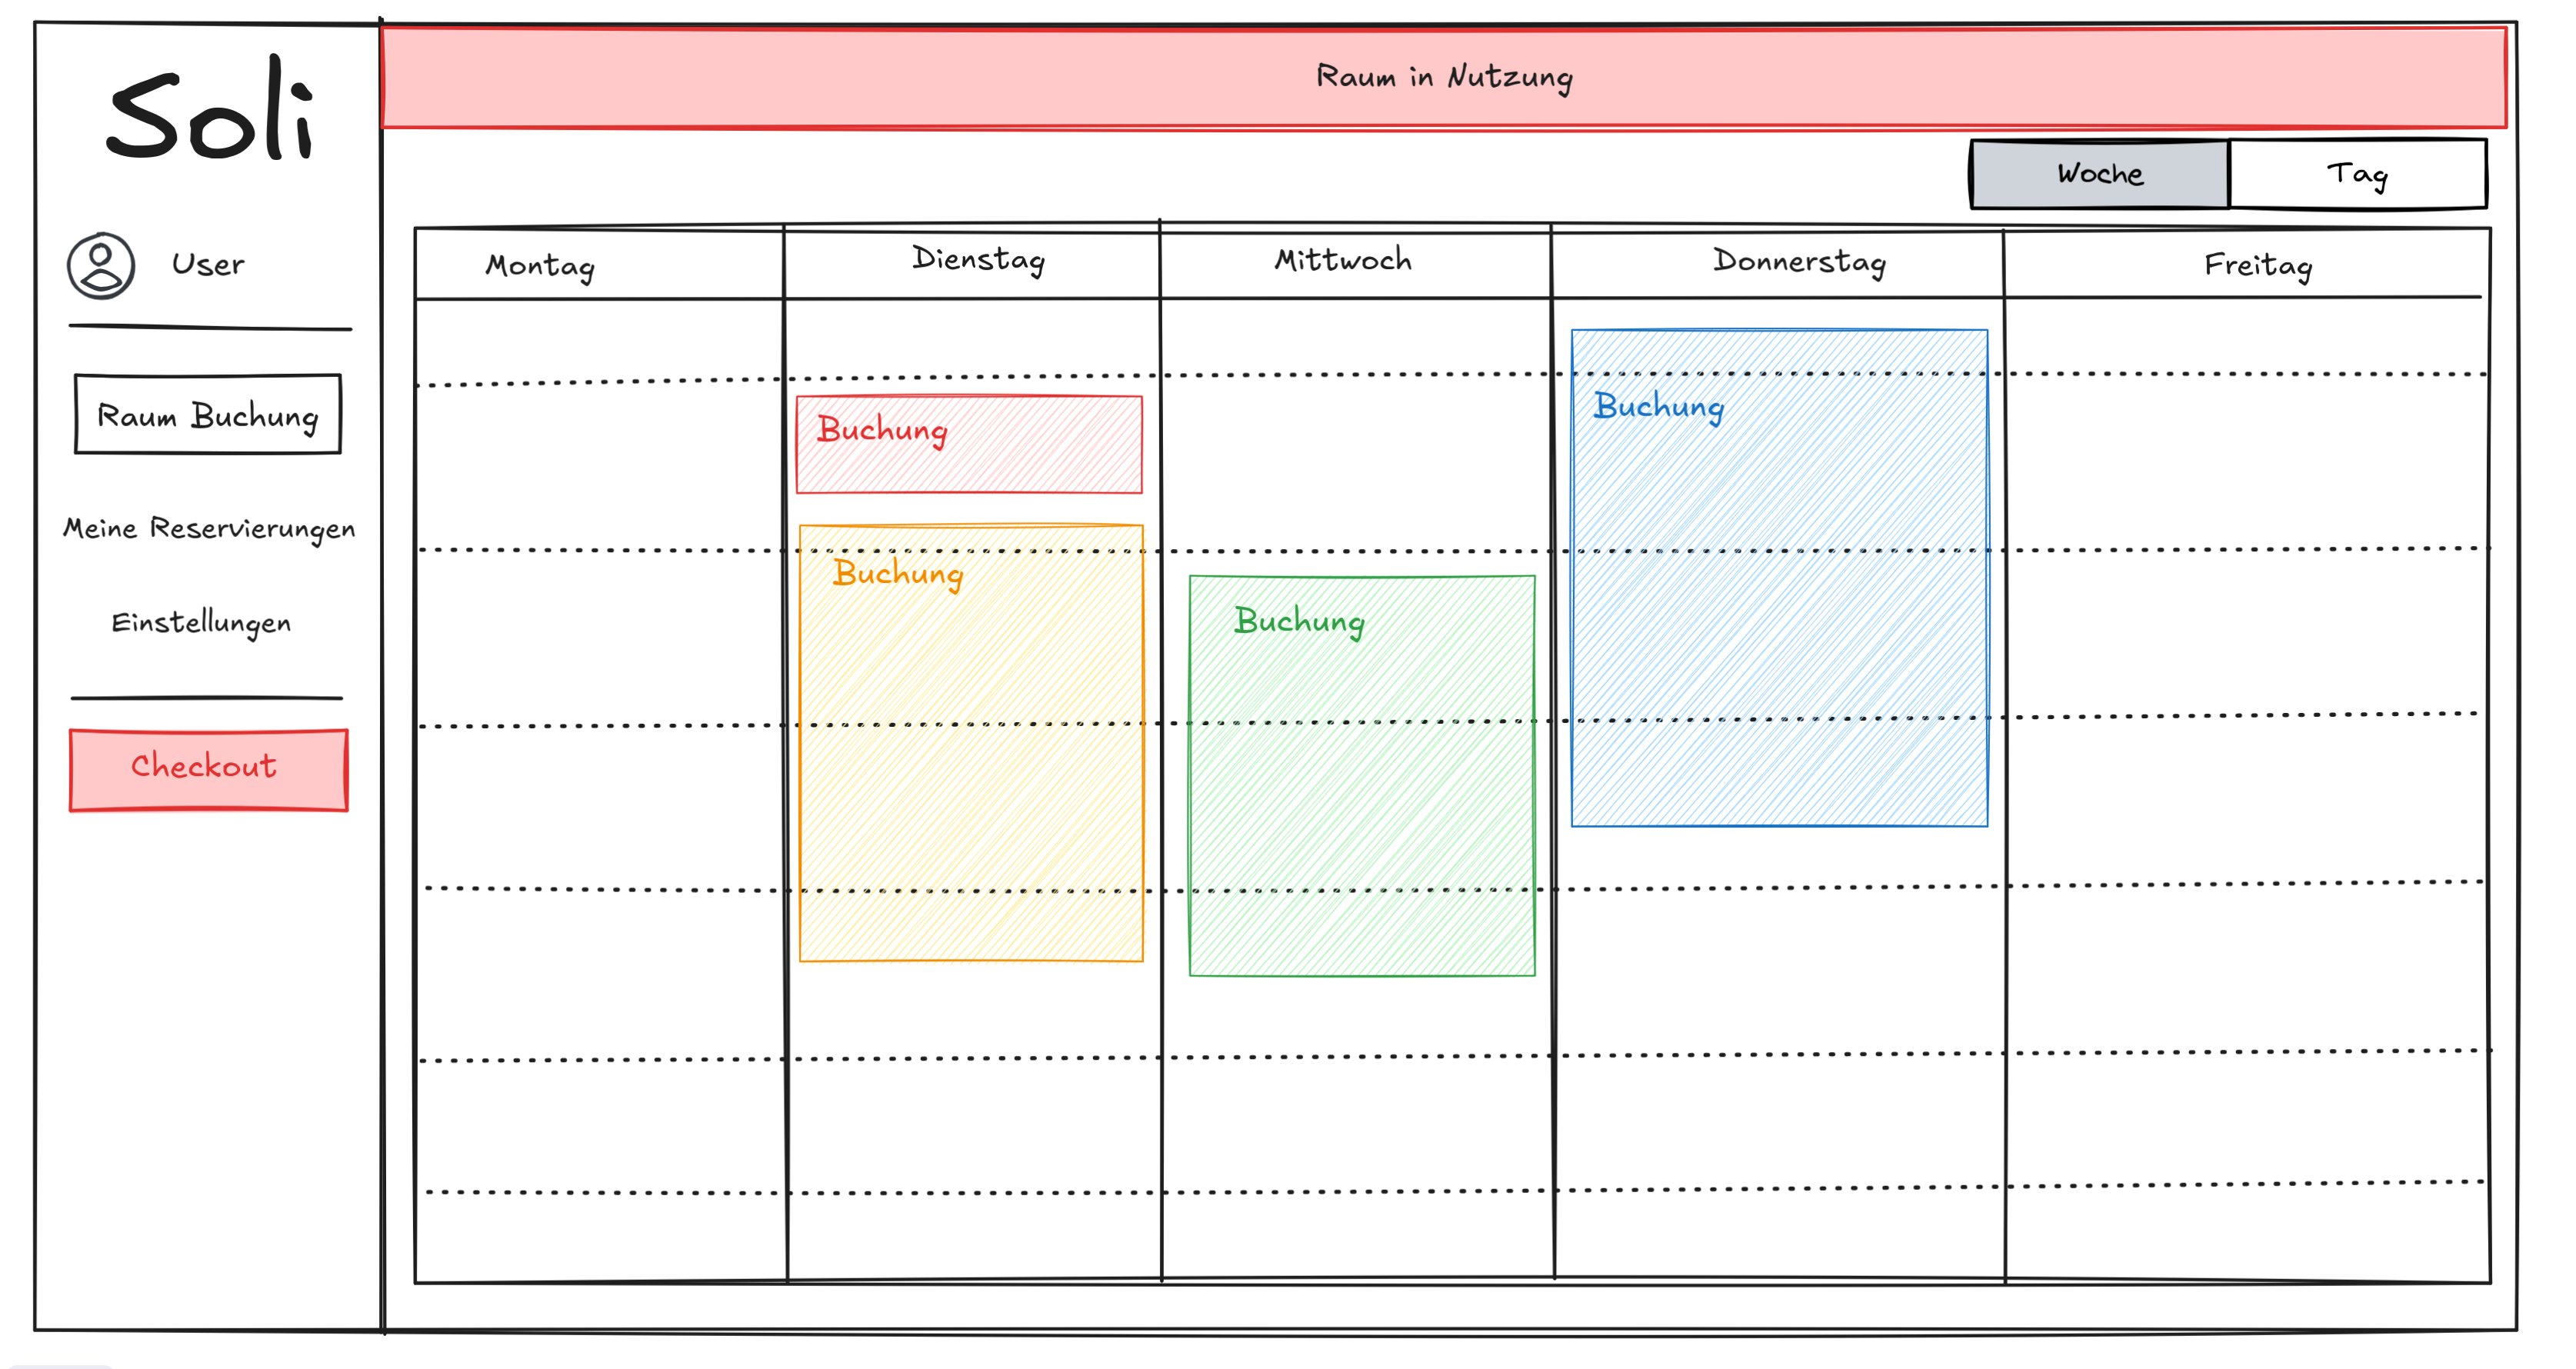
\includegraphics[width=\textwidth]{figures/mockup/checkout} % TODO Change this link to correct impl pic
    \caption{Implementierung: Quick Checkout}
    \label{fig:impl-checkout}
\end{figure}
\clearpage


\section{Terminübersicht}
Nutzende, die eine Buchung vorgenommen haben, können diese in der Terminübersicht,
die in Abbildung \ref{fig:overview} dargestellt ist, einsehen und verwalten.

Die Implementierung der Terminübersicht ist in \ref{fig:impl-overview} zu sehen und die der Terminansicht in \ref{fig:impl-calendarviewbooking}.

\begin{figure}[ht]
    \includegraphics[width=\textwidth]{figures/mockup/reservierungs��bersicht}
    \caption{Reservierungsübersicht}
    \label{fig:overview}
\end{figure}
\begin{figure}[ht]
    \includegraphics[width=\textwidth]{figures/mockup/reservierungs��bersicht} % TODO Change this link to correct impl pic
    \caption{Implementierung: Reservierungsübersicht}
    \label{fig:impl-overview}
\end{figure}
\clearpage
\begin{figure}
    \centering
    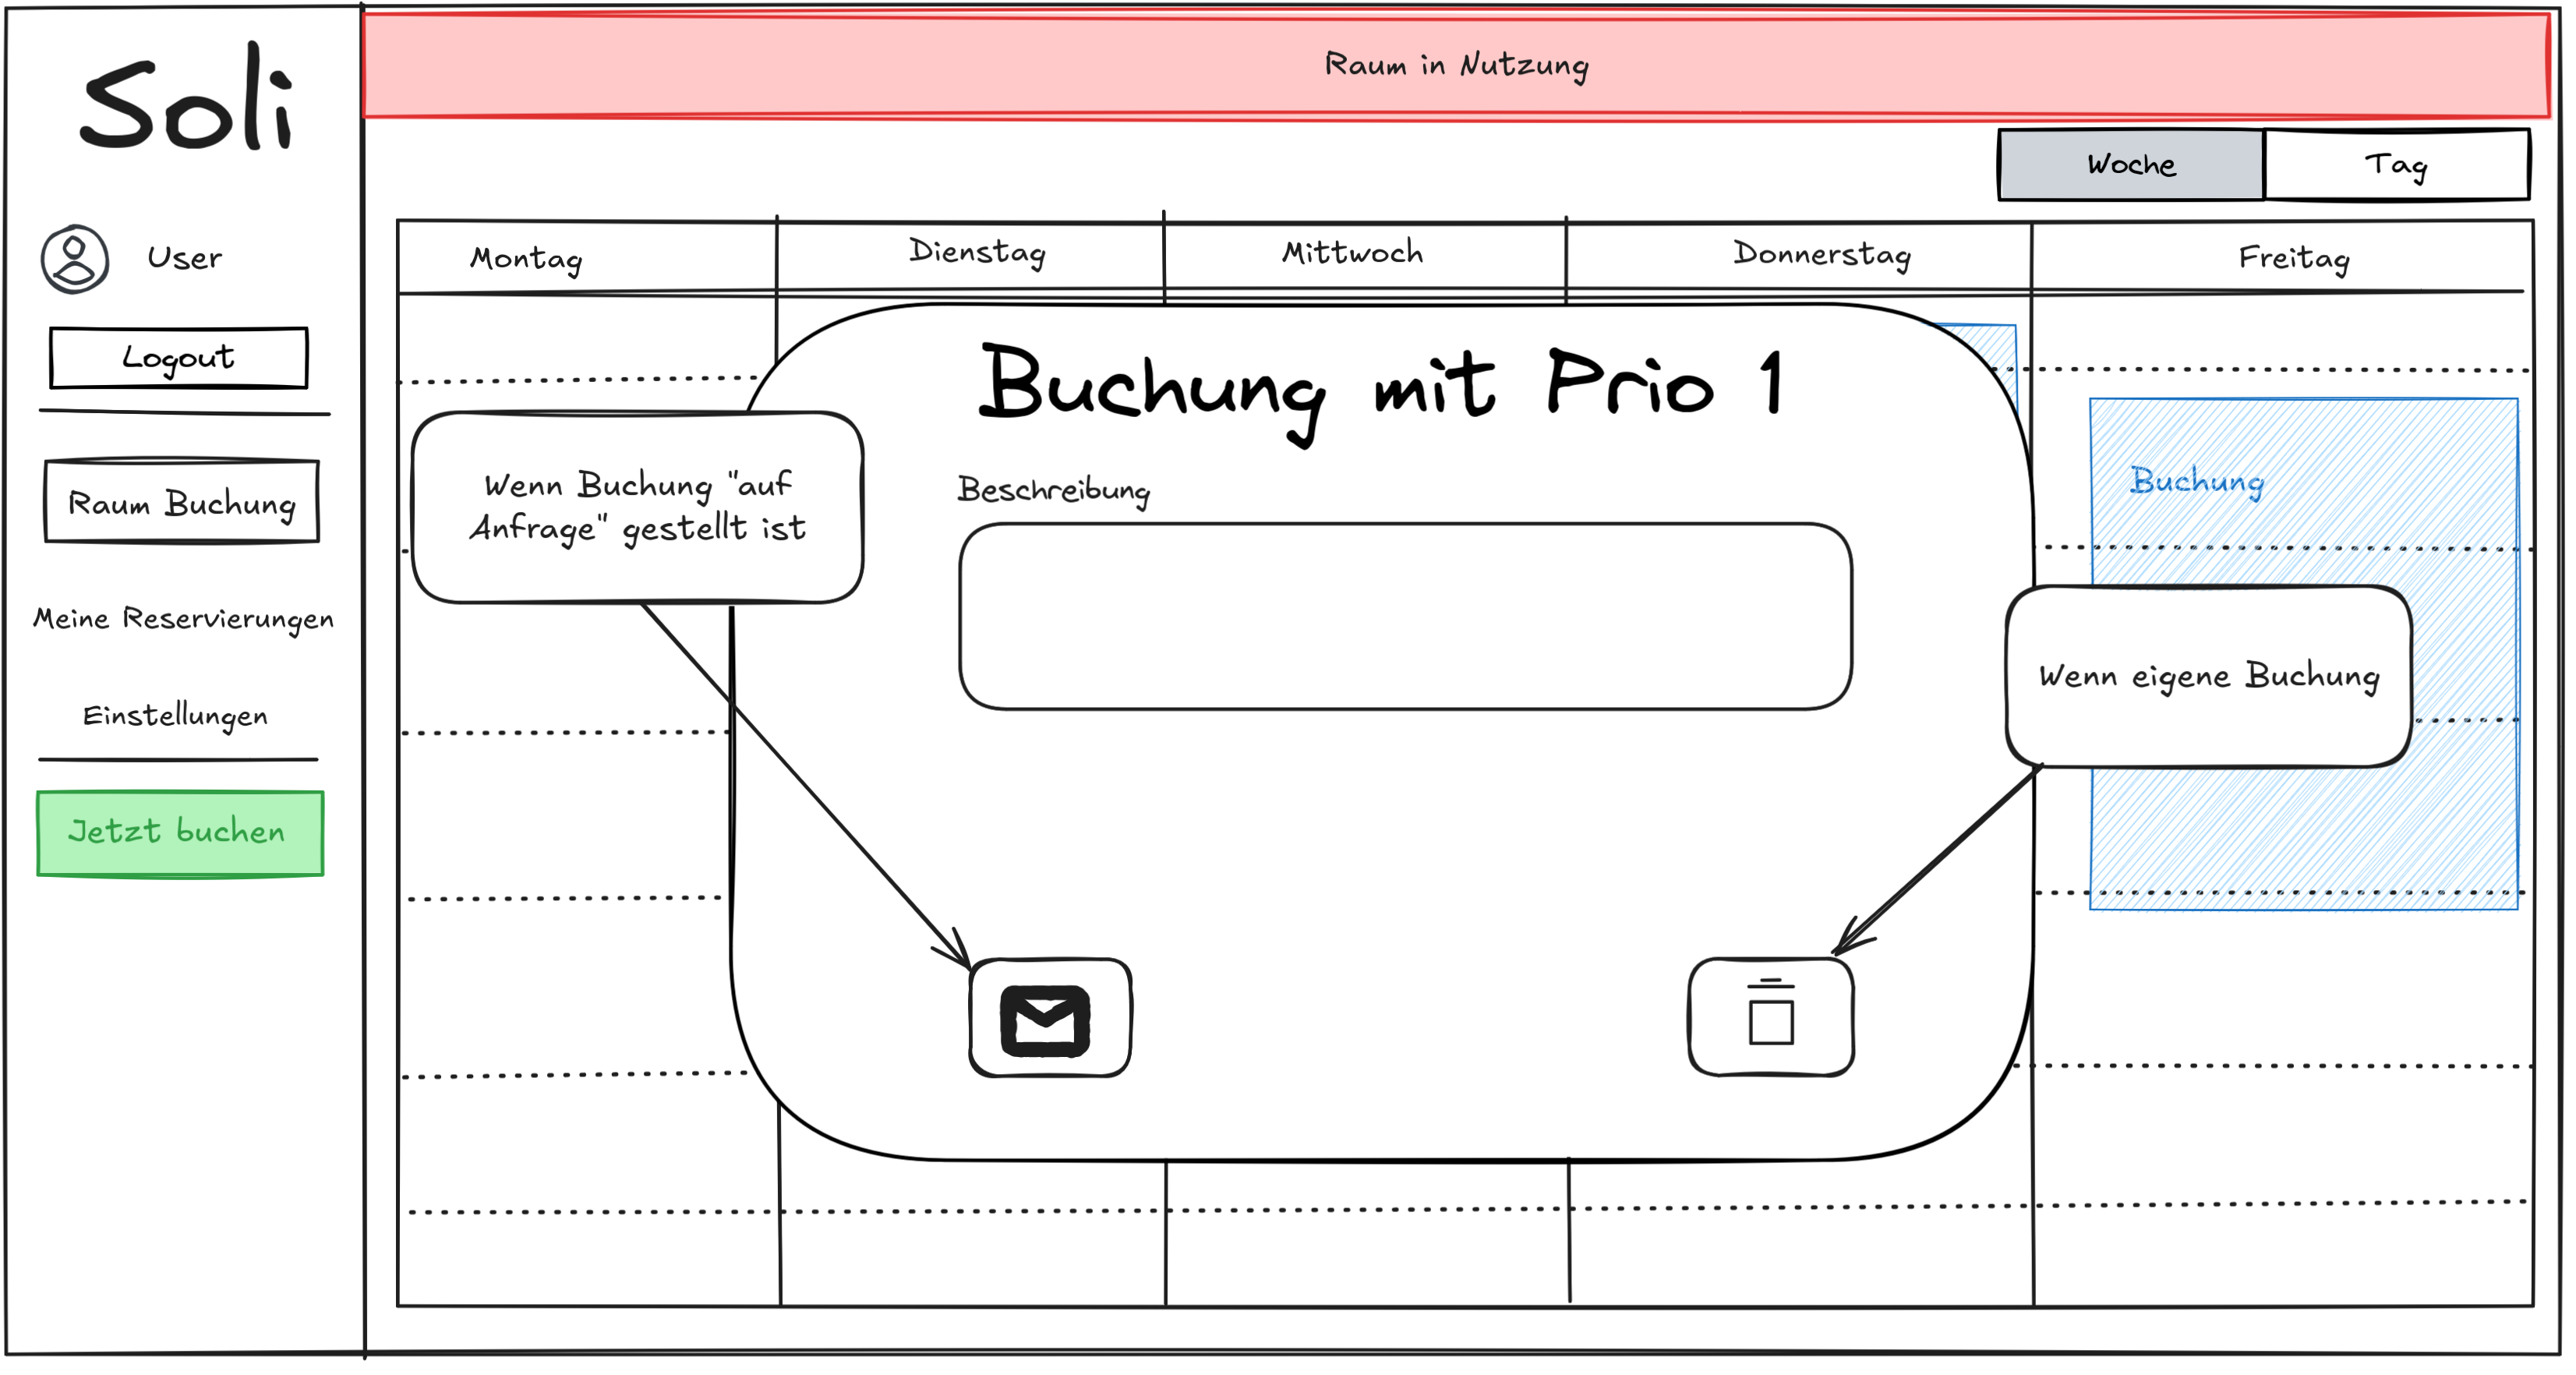
\includegraphics[width=\textwidth]{figures/mockup/reservierunginkalendar}
    \caption{Reserverierung im Kalender}
    \label{fig:calendarviewbooking}
\end{figure}
\begin{figure}
    \centering
    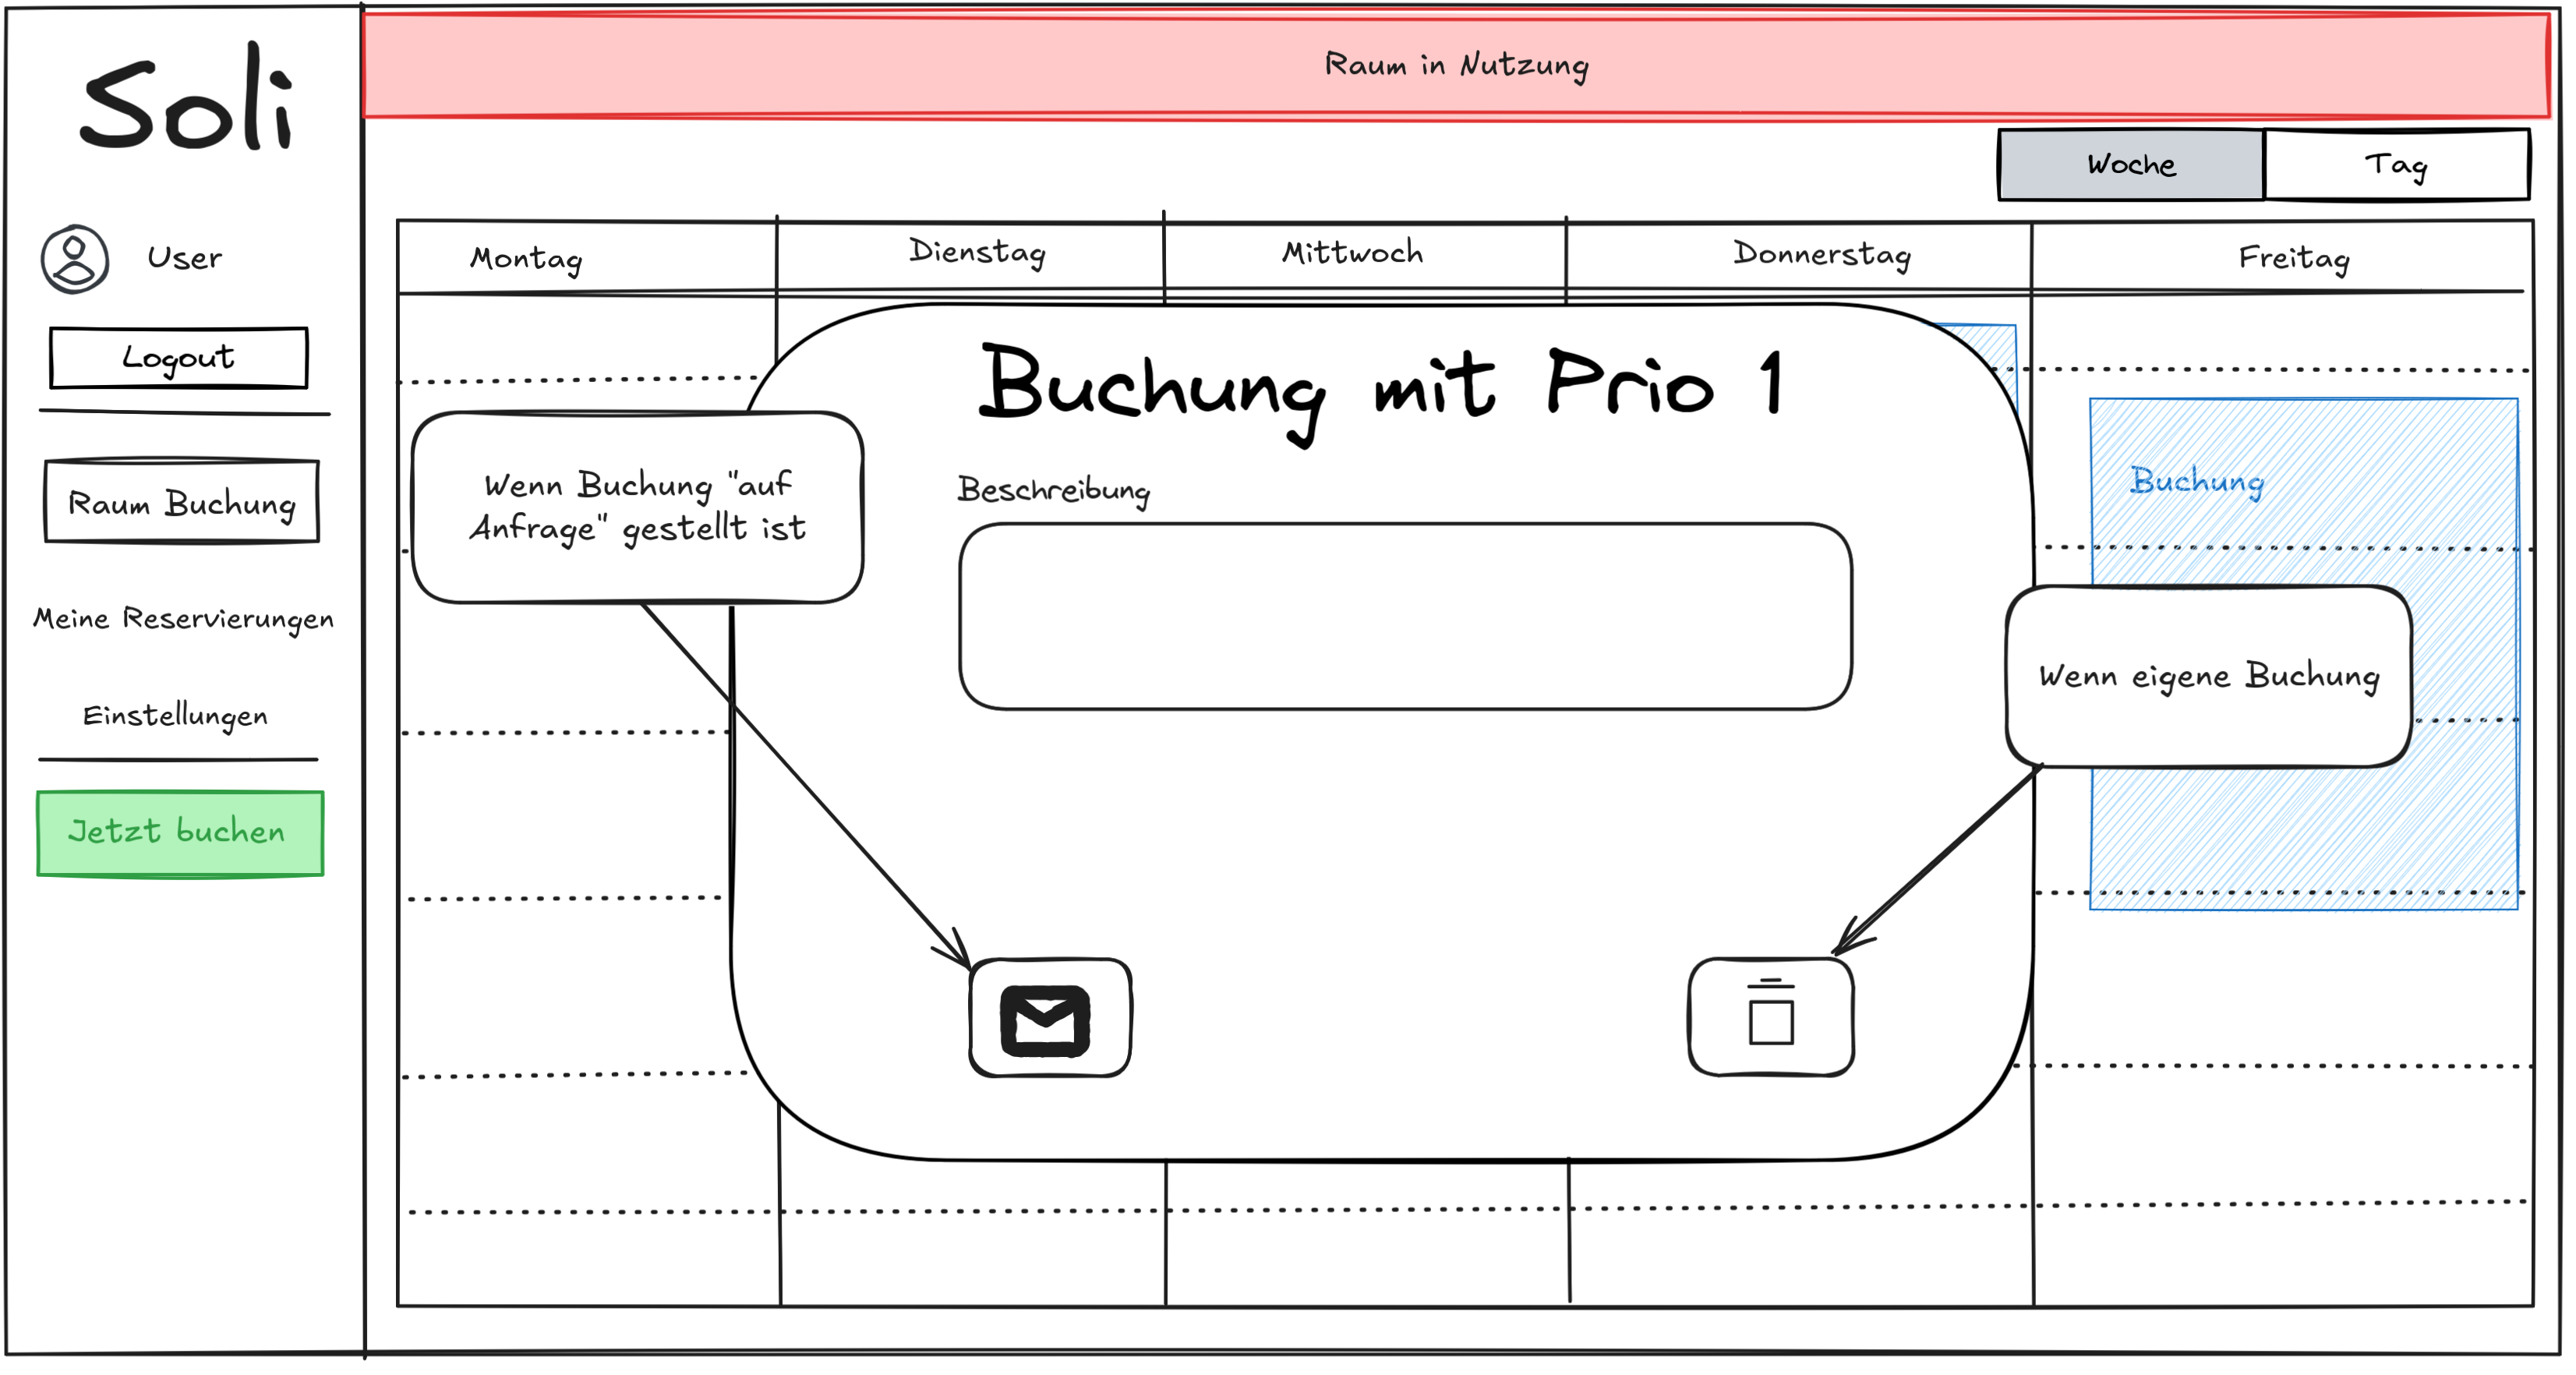
\includegraphics[width=\textwidth]{figures/mockup/reservierunginkalendar} % TODO Change this link to correct impl pic
    \caption{Implementierung: Reserverierung im Kalender}
    \label{fig:impl-calendarviewbooking}
\end{figure}
\clearpage


\section{Adminstration}
Ein/e Administrator*in hat die Möglichkeit, über die Benutzeradministrationsoberfläche, die in Abbildung \ref{fig:adminuser} dargestellt ist, Nutzende einzusehen und zu verwalten.

Die Implementierung der Kontenlsite ist in \ref{fig:impl-adminuser}

\begin{figure}[ht]
    \centering
    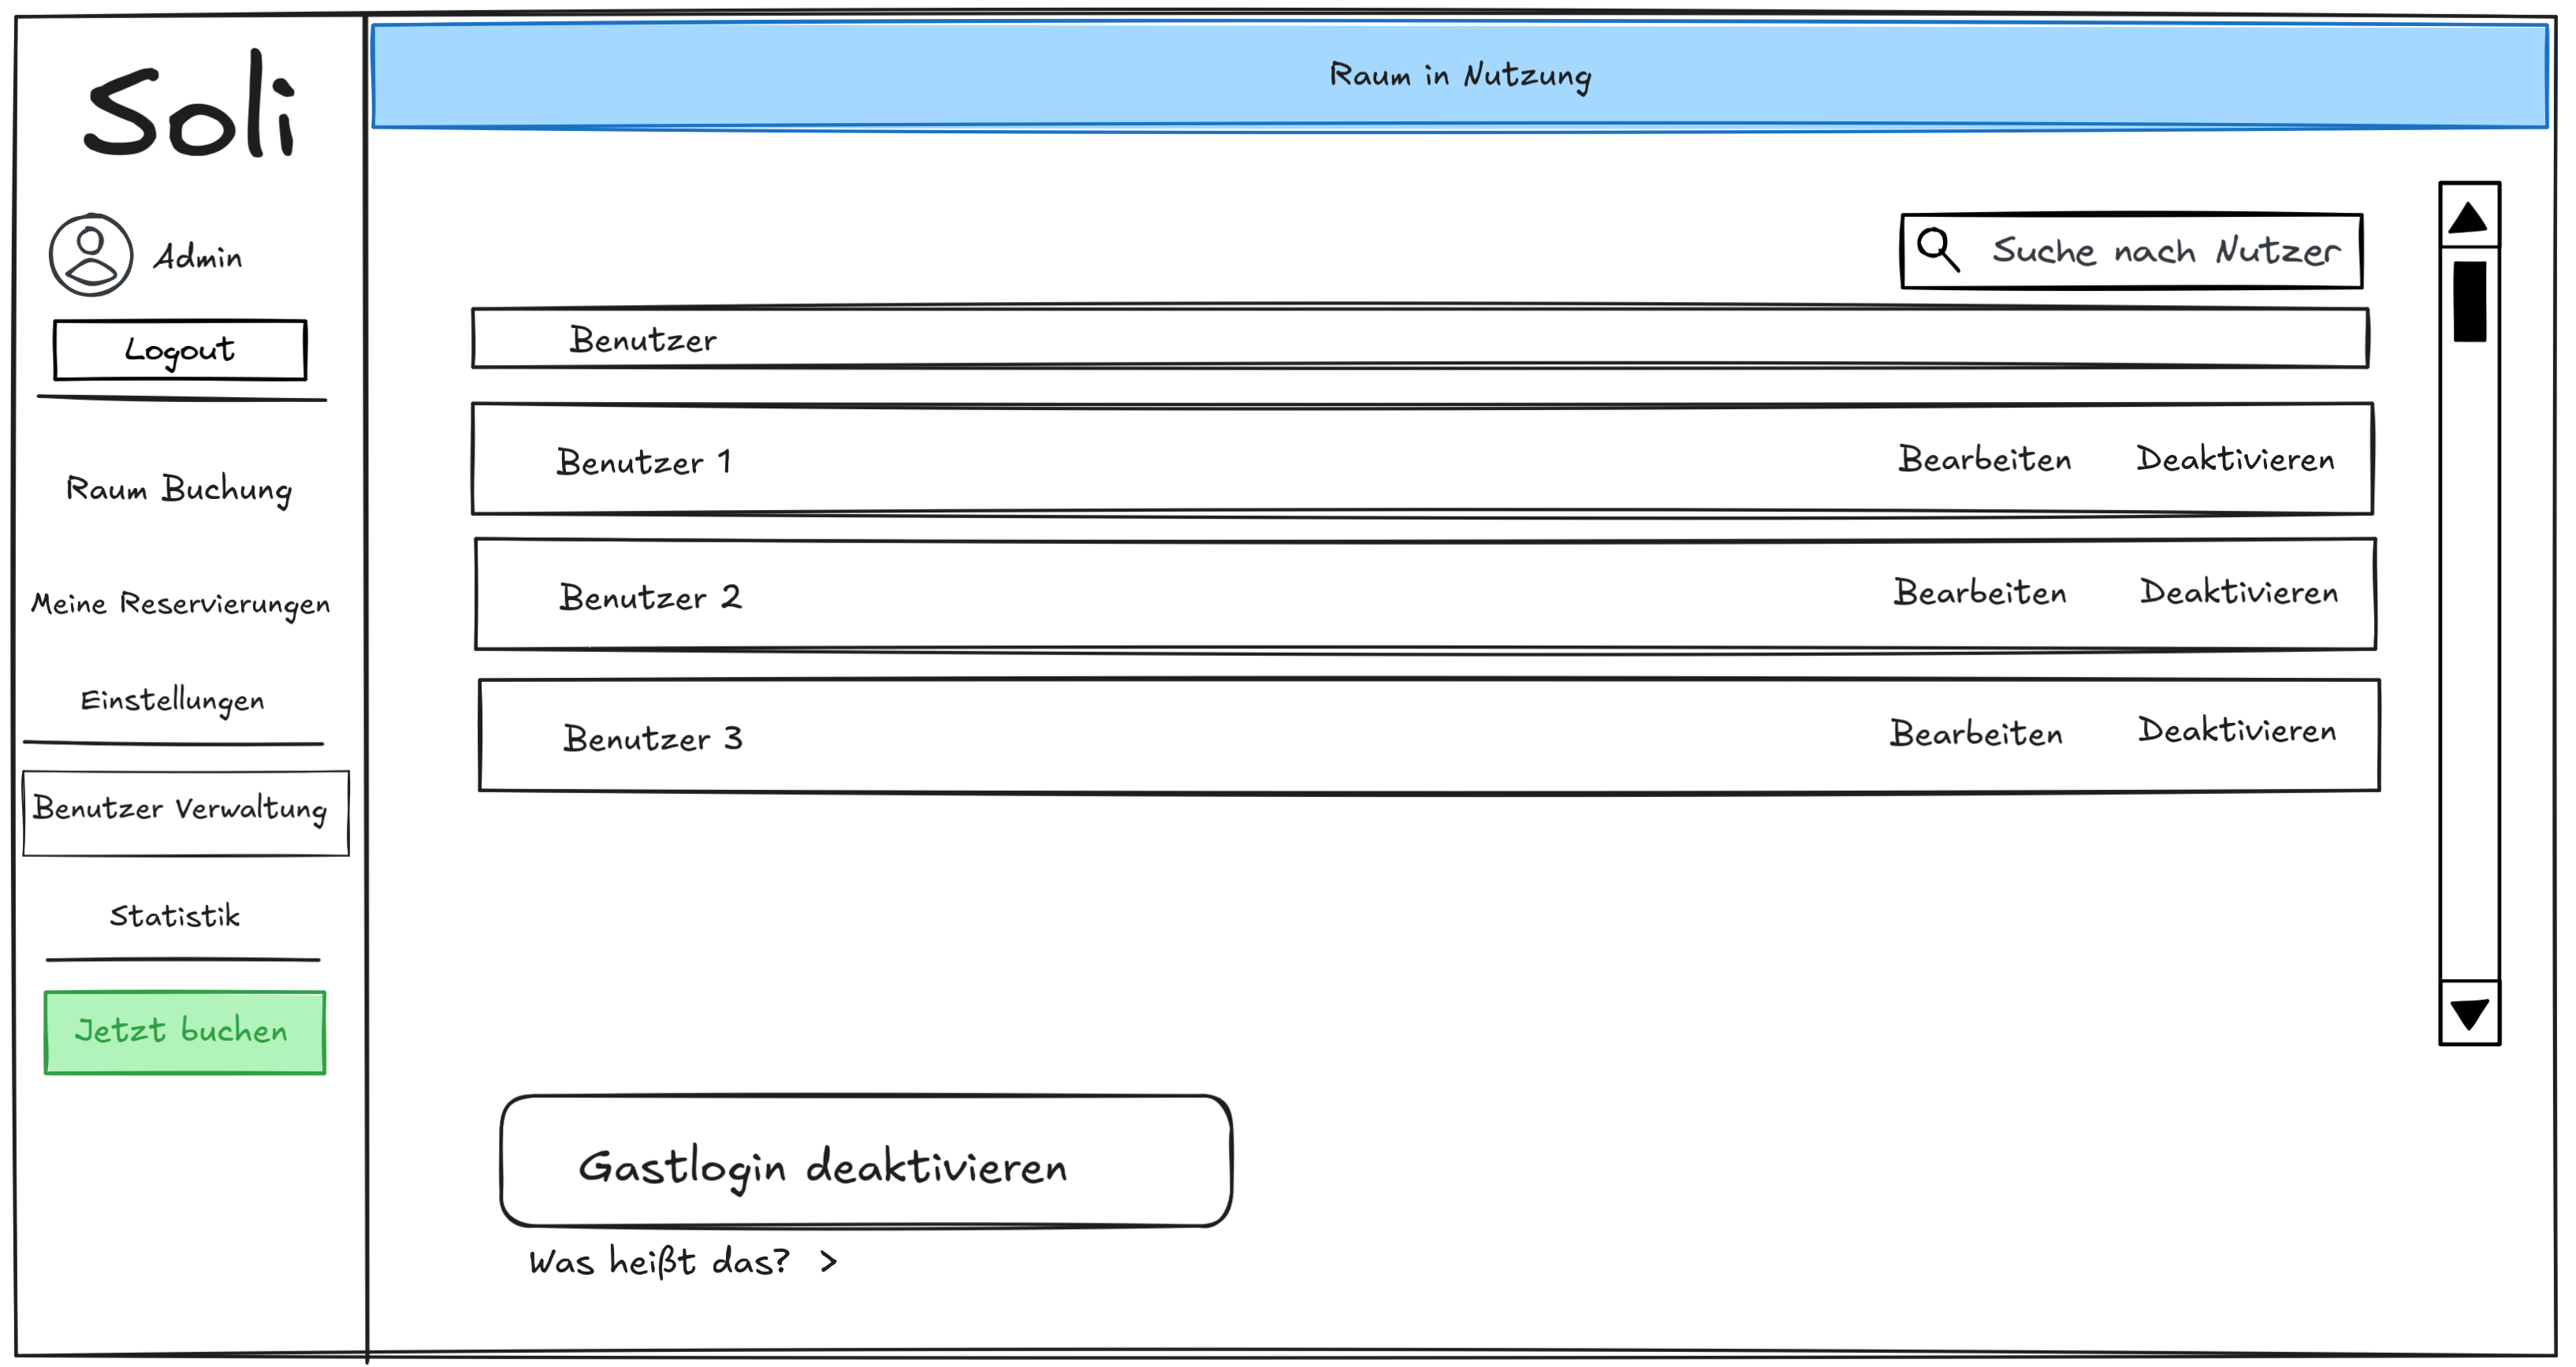
\includegraphics[width=\textwidth]{figures/mockup/useradminui}
    \caption{Benutzeradminstrationsoberfläche}
    \label{fig:adminuser}
\end{figure}
\begin{figure}[ht]
    \centering
    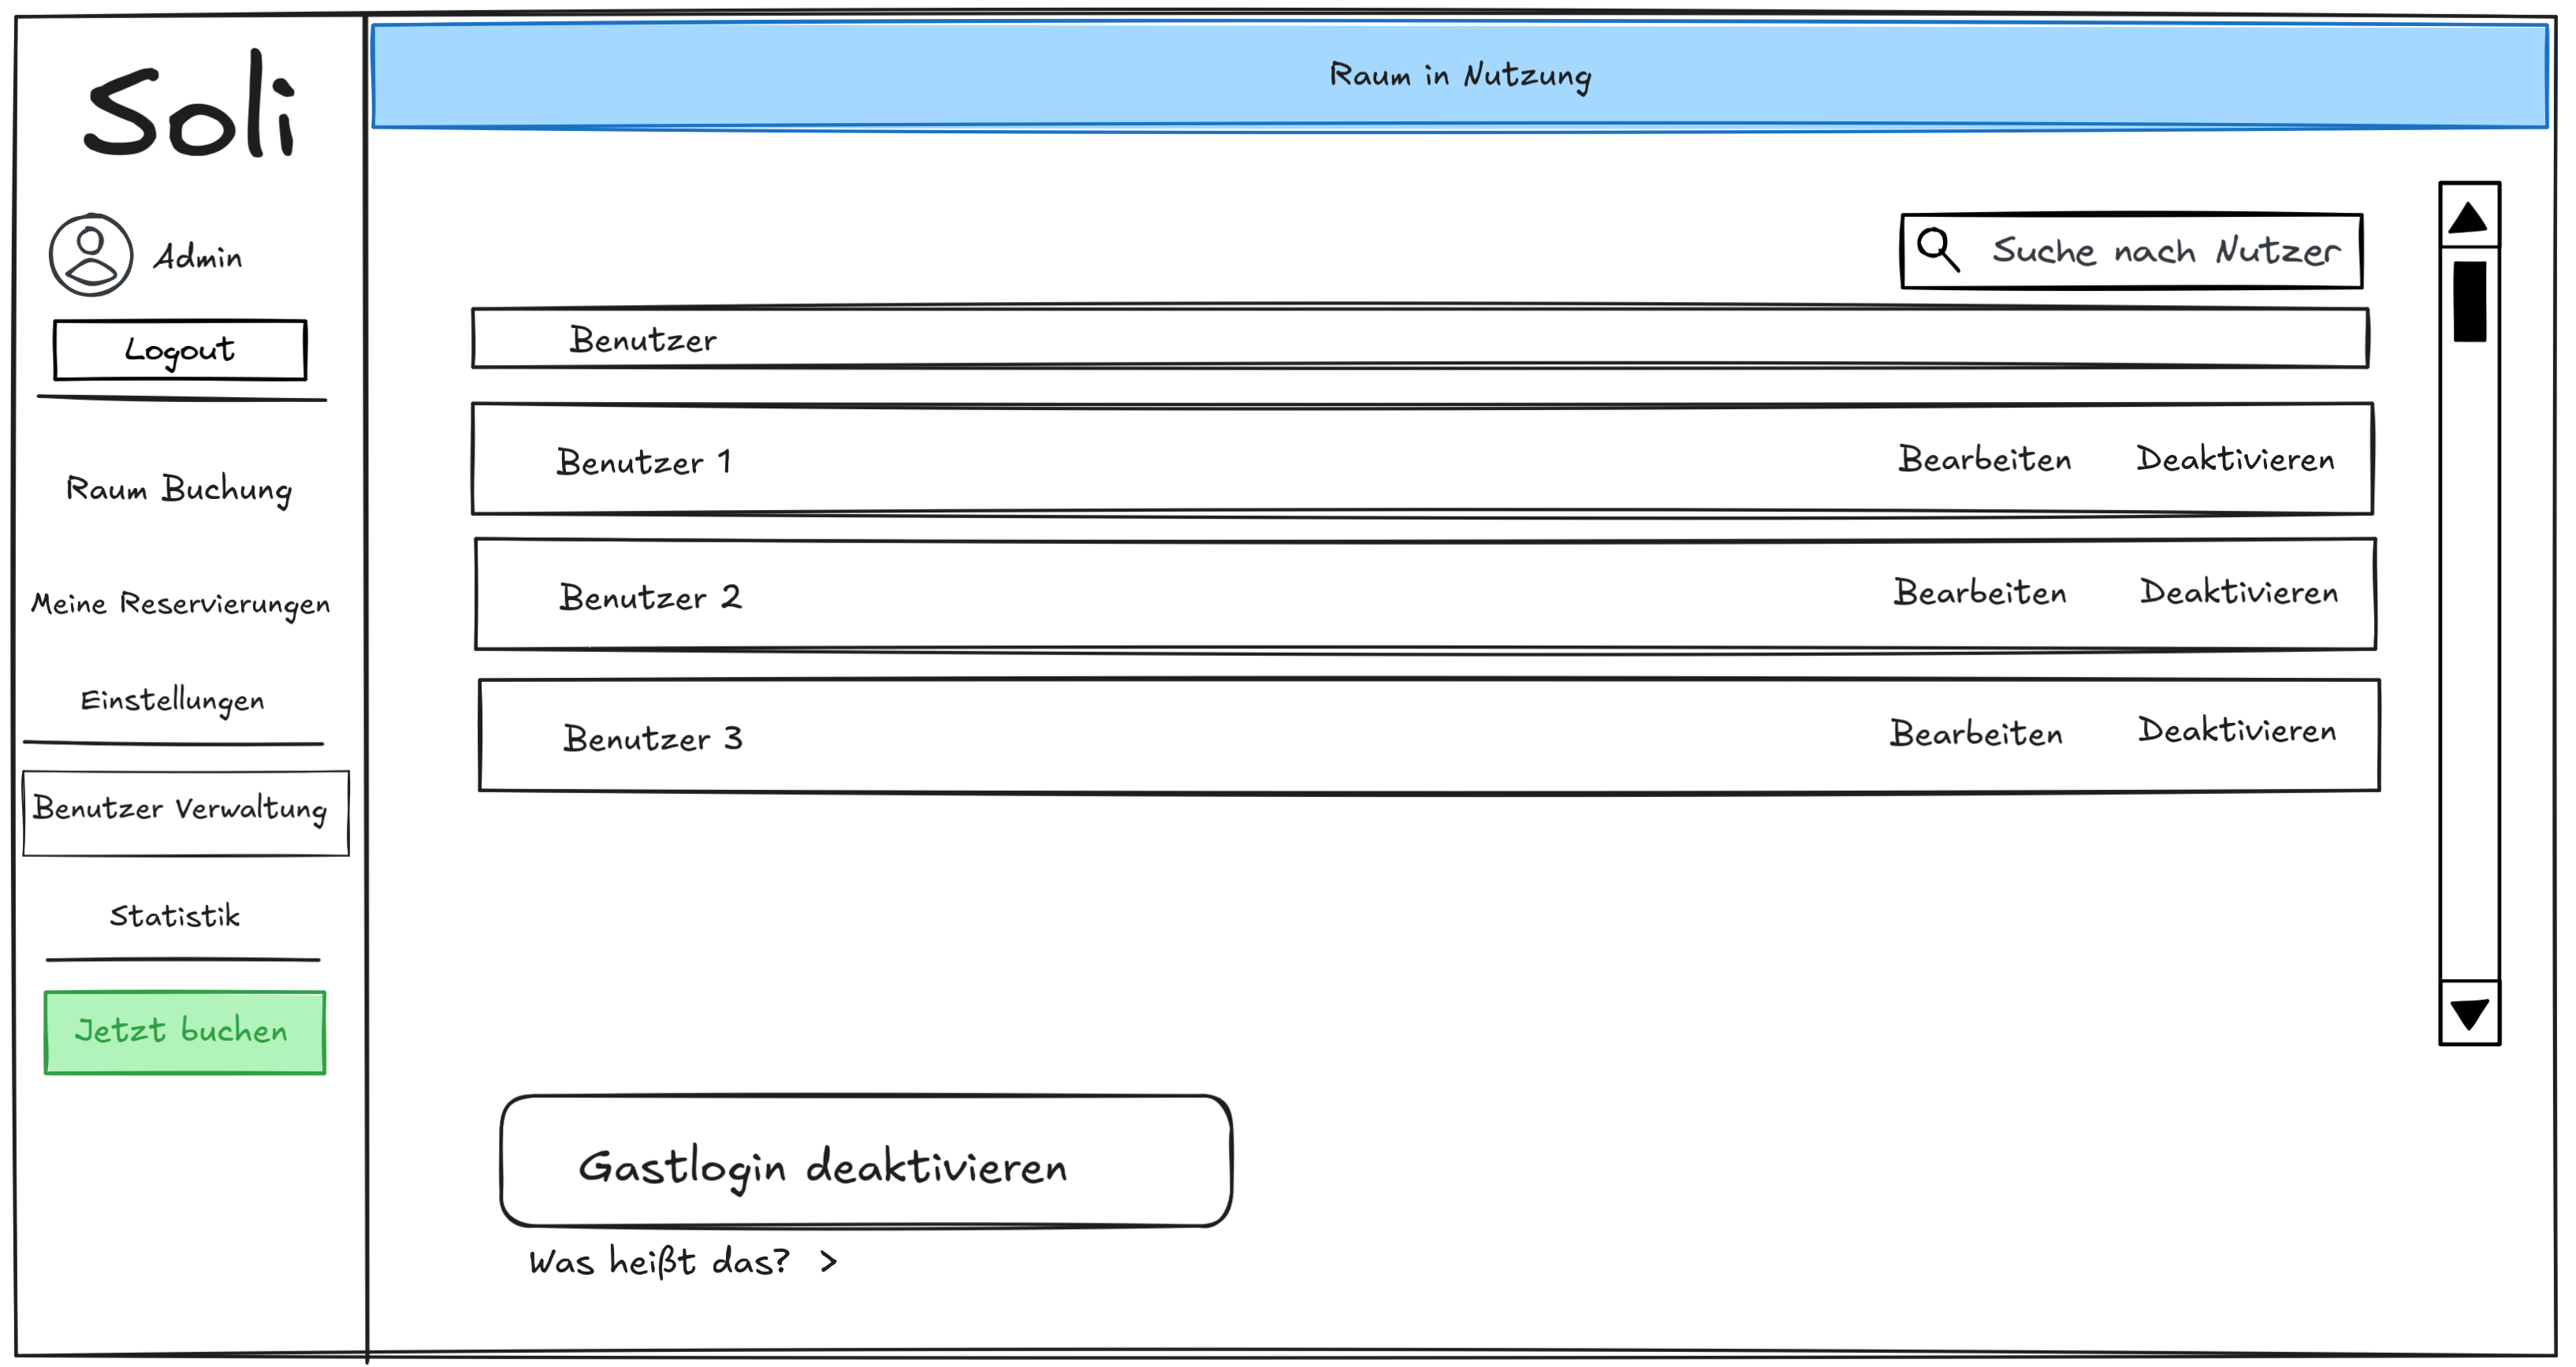
\includegraphics[width=\textwidth]{figures/mockup/useradminui} % TODO Change this link to correct impl pic
    \caption{Implementierung: Benutzeradminstrationsoberfläche}
    \label{fig:impl-adminuser}
\end{figure}
\clearpage

Die Funktionalität der einstellbaren Öffnungszeiten für einen Raum, welche nur von Administrator*innen genutzt werden kann
ist in seiner implementierten Form in \ref{fig:impl-adminopeninghours_config} zu sehen.

Die implementierte Visualisierung der Öffnungszeiten in der \textit{Kalender} Ansicht in \ref{fig:impl-adminopeninghours} zu sehen ist.

\begin{figure}[ht]
    \centering
    
\includegraphics[width=\textwidth]{figures/impl-views/placeholder} % TODO Change this link to correct impl pic
    \caption{Implementierung: Konfiguration}
    \label{fig:impl-adminopeninghours_config}
\end{figure}
\begin{figure}[ht]
    \centering
    
\includegraphics[width=\textwidth]{figures/impl-views/placeholder} % TODO Change this link to correct impl pic
    \caption{Implementierung: Visualisierung der Öffnungszeiten}
    \label{fig:impl-adminopeninghours}
\end{figure}
\clearpage

Die Implementierung des Wunschkriteriums einer Statistikansicht für ein/e Administrator*in ist in \ref{fig:impl-adminstatistic}

\begin{figure}[ht]
    \centering
    
\includegraphics[width=\textwidth]{figures/impl-views/placeholder} % TODO Change this link to correct impl pic
    \caption{Implementierung: Statistikansicht}
    \label{fig:impl-adminstatistic}
\end{figure}
% TODO more chapters
% TESTS?

\printglossaries

%------Ende des Dokumentes------------------------------------------------------
\end{document}
